% !TeX root = main
\documentclass[a4paper, 11pt]{article}

%------------------------------------------------------------------------------------
% import packages
\usepackage[scaled]{helvet}
%\usepackage{courier}
%\renewcommand\familydefault{\sfdefault} 

% Should include times new roman according to the slides
\usepackage{mathptmx}

% To use matrix
\usepackage{amsmath}

% To use mathbb
\usepackage{amssymb}

% To draw FSA
\usepackage{tikz}
\usetikzlibrary{automata,positioning,decorations.text,topaths,arrows.meta,decorations.pathmorphing,quotes}

\usepackage[T1]{fontenc}
\usepackage[english]{babel}
\usepackage{graphicx}
\usepackage{tabularx}
\usepackage{ltablex}
\usepackage{multirow}
\usepackage{subfig}
\usepackage{caption, booktabs}
\usepackage[hidelinks]{hyperref}
\usepackage[shortlabels]{enumitem}

% Font weight for pictures labels
\usepackage[labelfont=bf]{caption}

% No indent on new paragraphs
\usepackage[parfill]{parskip}

% Margins
\usepackage[margin=1in]{geometry}

% Set TOC Depth
\setcounter{tocdepth}{3}

% Left space
\usepackage{scrextend}

% code
\usepackage{listings}
\usepackage{color}
\definecolor{lightgray}{rgb}{.9,.9,.9}
\definecolor{darkgray}{rgb}{.4,.4,.4}
\definecolor{purple}{rgb}{0.65, 0.12, 0.82}
\lstdefinelanguage{Matlab}{
  keywords={typeof, new, true, false, catch, function, return, null, catch, switch, var, if, in, while, do, else, case, break, num2str},
  keywordstyle=\color{blue}\bfseries,
  ndkeywords={class, export, boolean, throw, implements, import, this, plot, linspace, numel, abs, semilogy, set, xlabel, ylabel, sqrt, all, isreal, chol, lu, eig, diag, spy, spdiags, sparse, sum, prod, cond, norm, eye, tril, inv, hilb, polyfit, polyval, interp1, interp2, spline, ones, zeros, log, loglog, diff},
  ndkeywordstyle=\color{orange}\bfseries,
  identifierstyle=\color{black},
  sensitive=false,
  comment=[l]{\%},
  morecomment=[s]{/*}{*/},
  commentstyle=\color{brown}\ttfamily,
  stringstyle=\color{red}\ttfamily,
  %morestring=[b]',
  morestring=[b]"
}

\lstset{
    language=Matlab,
    extendedchars=true,
    basicstyle=\footnotesize\ttfamily,
    showstringspaces=false,
    showspaces=false,
    %numbers=left,
    numberstyle=\footnotesize,
    numbersep=9pt,
    tabsize=2,
    breaklines=true,
    showtabs=false,
    captionpos=b,
    breaklines=true,
    morekeywords={matlab2tikz},
    keywordstyle=\color{blue},
    morekeywords=[2]{1}, keywordstyle=[2]{\color{black}},
    identifierstyle=\color{black},
    stringstyle=\color{mylilas},
    commentstyle=\color{mygreen},
    showstringspaces=false,%without this there will be a symbol in the places where there is a space
    %emph=[1]{for,end,break},emphstyle=[1]\color{red},
    emph=[1]{for,end,break},emphstyle=[1]\color{blue},
    frame=single
}

% functions with arrow
\newcommand{\f}[2]{\ensuremath{f:\,\,{#1}\rightarrow {#2}}}

% brackets
\newcommand{\brackets}[1]{\ensuremath{\{{#1}\}}}
\newcommand{\Brackets}[1]{\ensuremath{\begin{Bmatrix}
    {#1}
\end{Bmatrix}}}

% insieme quoziente
\newcommand{\bigslant}[2]{{\raisebox{.2em}{$#1$}\left/\raisebox{-.2em}{$#2$}\right.}}

% underlabel
\newcommand{\underlabel}[2]{\ensuremath{
    \underset{\text{#2}}{\underbrace{#1}}
}}

% mybox
\newcommand{\mybox}[1]{
    \fbox{\begin{minipage}{\linewidth}
        \vspace{1em}
        #1
        \vspace{1em}
    \end{minipage}}
}

\graphicspath{ {images/} }
\hypersetup{
    colorlinks,
    citecolor=black,
    filecolor=black,
    linkcolor=black,
    urlcolor=black
}

\begin{document}

\begin{titlepage}
	\centering
    \begin{tabular}{rl}
        Alessio Hu & (12345678)
    \end{tabular}

    \vspace{1.5cm}
    {\Huge \textbf{Numerical Analysis Summary\\}}
    \vspace{1.5cm}
    {\large 
        Numerical Analysis \\
        Prof. Perotto Simona \\ 
		 - Politecnico di Milano \par
    }
    \vspace{1.5cm}
    {\large \textbf{Something:}\\
    \vspace{0.5cm}
    Something else}
    \par
    \vspace{3cm}
    
\includegraphics[scale=0.4]{images/logo.pdf}
    \par
    \vspace{3cm}
	A.Y. 2022-2023
\end{titlepage}

\tableofcontents
    % !TeX root = ../main.tex

\section{Intro}
\subsection{Numerical Analysis and Errors}
M = Math\\
CS = Computer Science\\
E = Engineering

Numerical Analysis = M$\cap$CS\\
Basic methods to approach math problems

Scientific Computing = M$\cap$CS$\cap$E
Take a problem and replicate it on a digital device to understand better the situation

\begin{figure}[!ht]
    \begin{minipage}{\linewidth}
        \centering
        \makebox[\textwidth][c]{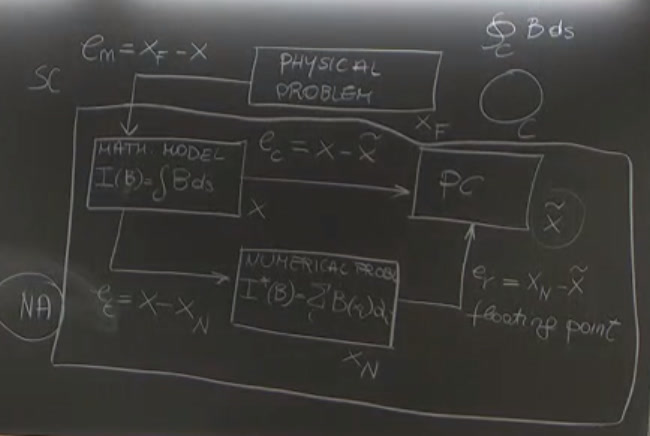
\includegraphics[width=1\textwidth]{images/Screenshot from 2022-09-21 15-28-17.png}}%
    \end{minipage}
\end{figure}
Where:
$$
\begin{cases}
    x_F\text{ solution of physical model}\\
    x\text{ solution of mathematical model}\\
    \tilde{x}\text{ does not substitute reality simulation}\\
\end{cases}
$$
We replaced the integral with a summation, ia PC there is no concept of infinity.\\
What to do after we observe what's going on? Use a better model or a better $x\leftrightarrow\tilde{x}$ mapping.

Errors:
$$
\begin{cases}
    e_m=x_F-x\text{ modelling error between physical problem and mathematical model}\\
    e_c=x-\tilde{x}\text{ computational error}=e_t+e_r
    \begin{cases}    
        e_t=x-x_N\text{ truncation error}\\
        e_r=x_N-\tilde{x}\text{ rounding error, floating point approximation}
    \end{cases}
\end{cases}
$$

Kinds of errors:
\begin{itemize}
    \item $|x-\tilde{x}|$\\
    \textbf{Absolute error}, $|e_c|$. Consider absolute error based on model
    \item $\frac{|x-\tilde{x}|}{|x|}$\\
    \textbf{Relative error}, more meaningful, like percentage
\end{itemize}

\subsection{Floating point representation}
    % !TeX root = ../main.tex

\section{Nonlinear equations}

$f$, we want to find $\alpha\in\mathbb{R}$ zero of $f$ such that $f(\alpha)=0$

It is not easy to find the zero of a function when
$\mathbb{P}_n\,\,n>4$. From here we need to approximate the zeros of a nonlinear function.

An example of physical phenomenol: the ideal gas equation:
$$pV=nRT$$
To find $V$
$$\left[
    p+a\left(
        \frac{N}{V}
    \right)^2
\right](V-Nb)=kNT$$
A nonlinear equation, although we know the pressure, the temperature and the constants $a$ and $k$, it is not easy to solve.

We use \textbf{iterative methods}
$$\underlabel{x^{(0)}}{Initial guess}$$

\begin{figure}[!ht]
    \begin{minipage}{\linewidth}
        \centering
        \makebox[\textwidth][c]{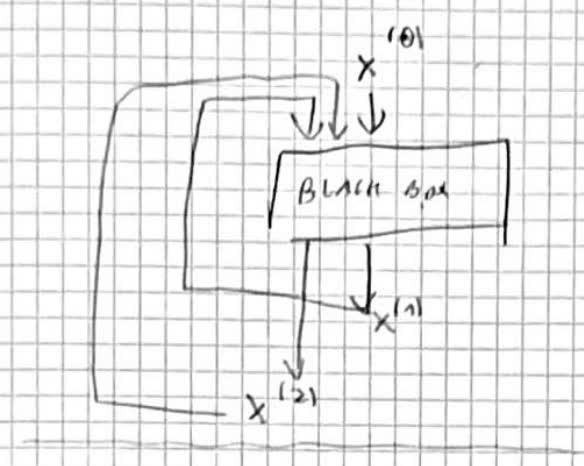
\includegraphics[width=0.5\textwidth]{images/Screenshot from 2022-09-20 22-39-23.png}}%
        %\caption{Black box}
        %\label{BarsNielsenCrop}
    \end{minipage}
\end{figure}

$$x^{(k)}\simeq\alpha$$
Ideally I want
$$\lim_{k\rightarrow\infty}x^{(k)}=\alpha$$
\textbf{Convergence}, or equivalently
$$e^{(k)}=\alpha-x^{(k)}$$
$$\lim_{k\rightarrow\infty}e^{k}=0$$
But we have to decide when to stop this approximation, \textbf{stopping criteria}: set a maximum number of iterations and a tolerance error.

We are looking at the approximation error
$$?\,\,\alpha\in\mathbb{R}\,\,s.t.\,\,\underlabel{f(\alpha)=0}{non linear}$$
Two methods: bisection and Newton method

\subsection{Bisection method}
In mathematics, the bisection method is a root-finding method that applies to any continuous function for which one knows two values with opposite signs.\\
We first have to fix the hypothesis, which coincides on the hypothesis of the zero of nonlinear continuous functions:
\begin{enumerate}
    \item $f\in C^0([a,b])$\\
    Set of all continuous functions in $[a,b]\subset\mathbb{R}$
    \item $f(a)f(b)<0$\\
    \begin{figure}[!ht]
        \centering
        \subfloat[][\centering The example has more zeros even, this is too much for us, even one is enough]{{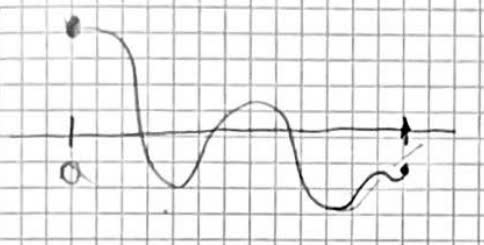
\includegraphics[width=7cm]{images/Screenshot from 2022-09-20 22-39-38.png} }}%
        \qquad
        \subfloat[][\centering The function is taking values at opposite sign at endpoints, which means that the function $f$ has at least one zero in the interval]{{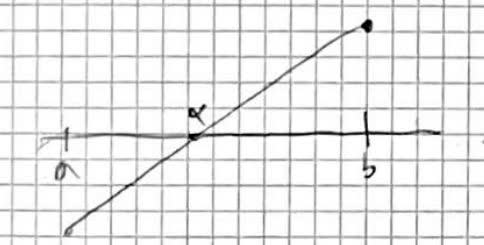
\includegraphics[width=7cm]{images/Screenshot from 2022-09-20 22-39-42.png} }}%
        \captionsetup{justification=centering}
    \end{figure}
\end{enumerate}

Starting from an interval, we shrink it:
$$
\alpha\in I^{(0)}=[a,b]$$
$$
\alpha\in I^{(1)}\subset I^{(0)}$$
$$
|I^{(0)}|=\frac{|I^{(0)}|}{2}$$
$$
\alpha\in I^{(2)}\subset I^{(1)}$$
$$
|I^{(2)}|=\frac{|I^{(1)}|}{2}$$
$$
\vdots
$$

Collection of intervals that are getting smaller and smaller, that all contain $\alpha$ (the zero), so at the end we will get to $\alpha$

Strength point of bisection: \textbf{always convergent, but has a lot of drawbacks too}.

But we are looking for $x^{(k)}$ that approximates $\alpha$
$$?\,\,x^{(k)}\simeq\alpha$$
To do this we consider the midpoint of the interval

\begin{figure}[!ht]
    \begin{minipage}{\linewidth}
        \centering
        \makebox[\textwidth][c]{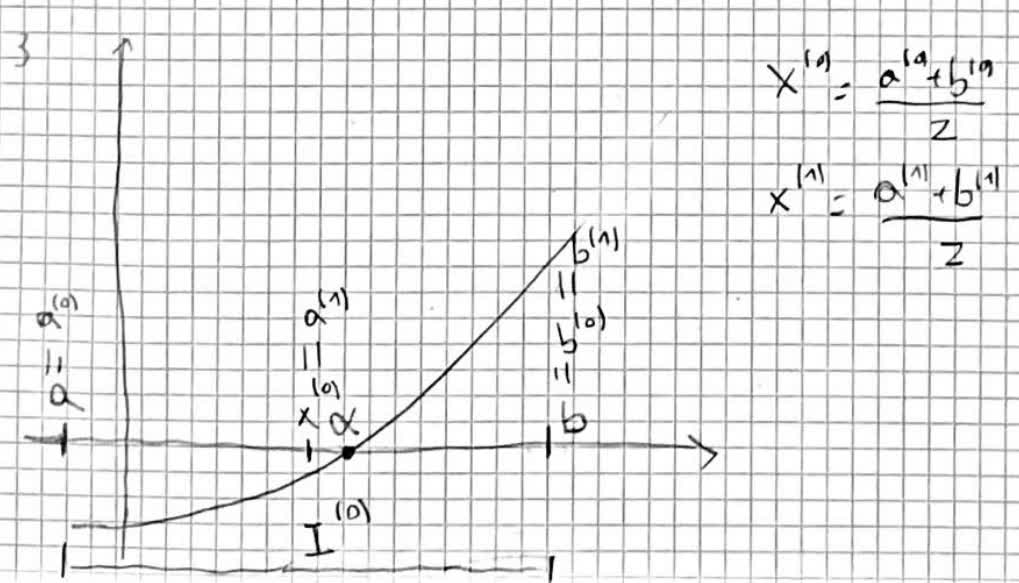
\includegraphics[width=0.8\textwidth]{images/Screenshot from 2022-09-20 22-39-51.png}}%
        %\caption{Function 3}
        %\label{BarsNielsenCrop}
    \end{minipage}
\end{figure}

We see that in this example the first midpoint is already close to $\alpha$. Now we have to choose a new subinterval $I^{(1)}$, we will choose the right subinterval as we need to satisfy the hypothesis that the extremes have opposite signs. We then continue iteratively.

The algorithm is similar to binary search. Formally:\\
\textbf{Inputs}: $a=a^{(0)},\,\,b^{(0)}=v,\,\,f;\,\,TOL,\,\,Nmax$\\
Where $TOL$ is the tolerance and $Nmax$ the maximum number of iterations.

\begin{center}
    \begin{lstlisting}[escapeinside=`']
        while(true)
            `$x^{(k)}=(a^{(k)}+b^{(k)})/2$'
            if(`$f(x^{(k-1)})=0$') break;
            if `$f(a^{(k-1)})f(x^{(k-1)})<0$'
                `$a^{(k)}=a^{(k-1)},b^{(k)}=x^{(k-1)}$';
            else
                `$a^{(k)}=x^{(k-1)},b^{(k)}=b^{(k-1)}$';
            end
        \end{lstlisting}
\end{center}

Regarding the intervals, we see that:
$$
|I^{(k)}|=\frac{b-a}{2^k}=\frac{|I^{(0)}|}{2^k}
$$
$$
|e^{(k)}|=|\alpha-x^{(k)}|<\frac{|I^{(k)}|}{2}=\frac{b-a}{2^{k+1}}
$$
$$
\lim_{k\rightarrow\infty}|e^{(k)}|=(b-a)\lim_{k\rightarrow\infty}\left(\frac{1}{2}\right)^{(k+1)}=0
$$
Regarding the tolerance
$$
?\,\,k\text{ s.t. }|e^{(k)}|\leq TOL=10^{-9}
$$
$$
\frac{b-a}{2^{(k+1)}}\leq TOL
$$
$$
\frac{b-a}{TOL}\leq 2^{(k+1)}
$$
$$
\log_2\left(
    \frac{b-a}{TOL}
\right)\leq k+1
$$
$$
k\geq\log_2\left(
    \frac{b-a}{TOL}
\right)-1
$$
The right member will represent the $Nmax$
$$
Nmax=\left\lceil\log_2\left(
    \frac{b-a}{TOL}
\right)\right\rceil=
\left\lceil\log_{10}\left(
    \frac{b-a}{TOL}
\right)/\log_{10}2\right\rceil
$$

\subsubsection{Pros and Cons}
Pros:
\begin{itemize}
    \item Converges
    \item Can compute maximum number of iterations
\end{itemize}
Cons:
\begin{itemize}
    \item We are losing the monotonicity of the method, a subsequent guess is not guaranteed to find a $x$ closer to $\alpha$ w.r.t. the previous $x$, \textbf{not monotonic w.r.t. to error, the error does not necessarily decreases at each step, we have no convergence order}
    \item Cannot find $\alpha$ in a single step
    \item We are only exploiting the fact that the function is changing sign, function values of $f$ are ignored
\end{itemize}

\subsection{Newton method}
$Nmax$ has to hold for all continuous functions in that interval $[a,b]$, so it has to be large.

The Newton we are not only exploiting the sign of f, but also the values. It is the most powerful method, and demands that:
$$f\in C^1([0,0])$$
Set of functions continuous in their first derivative

Replace $f$ with the tangent line at point of oure initial guess $x^{(0)}$, then take the intersection of the tangent with the $x$ axis, that will be our $x^{(1)}$. Then repeat:

\begin{figure}[!ht]
    \begin{minipage}{\linewidth}
        \centering
        \makebox[\textwidth][c]{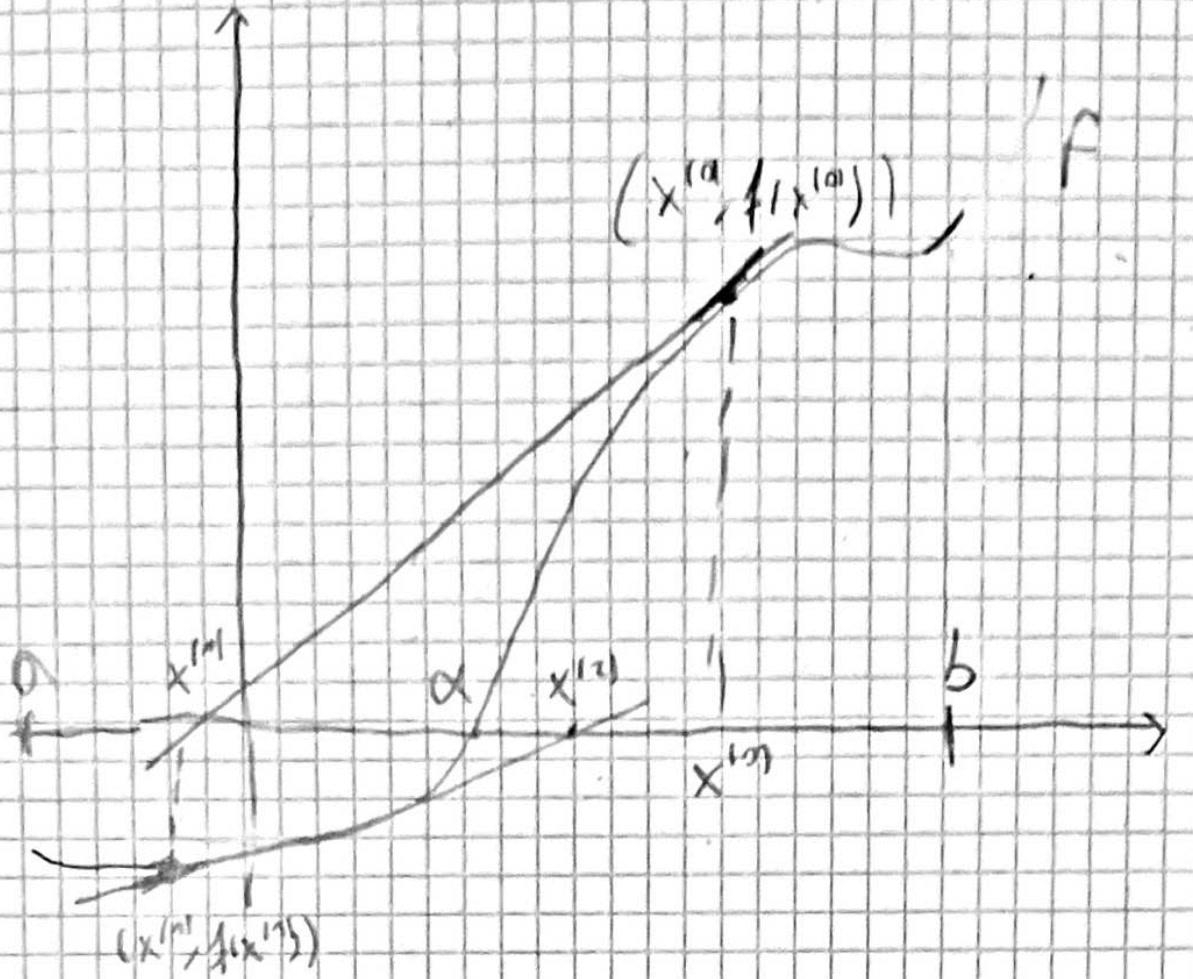
\includegraphics[width=0.8\textwidth]{images/Screenshot from 2022-09-20 22-40-09.png}}%
        %\caption{Tangent Newton method}
        %\label{BarsNielsenCrop}
    \end{minipage}
\end{figure}
tg to $f$ at $(x^{(k)},f(x^{(k)}))\\
y(x)=f(x^{(k)})+f'(x^{(k)})(x-x^{(k)})\\
x^{(k+1)}\text{ s.t. }y(x^{(k+1)})=0\\
f(x^{(k)})+f'(x^{(k)})(x^{(k+1)}-x^{(k)})
$\\
From this equality we want to derive $x^{(k+1)}$:\\
$$x^{(k+1)}=x^{(k)}-\frac{f(x^{(k)})}{f'(x^{(k)})}\qquad k\geq 0$$
Assuming $f'(x^{(k)})\neq 0$\\
It can be proved that this algorithm is just a truncation of the Taylor expansion
\subsubsection{Taylor expansion}
We must first decide the center and where to evaluate the expansion. In oure case the center is $x^{(k)}$, we evaluate at $x^{(k+1)}$
$$f(x)=f(x^{(k)})+f'(x^{(k)})(x-x^{(k)})+O\left((x-x^{(k)})^2\right)x^{(k+1)}$$
So if we evaluate at $x^{(k+1)}$, we simply replace $x$. We neglect the big $O$ term and if $k$ is sufficiently large, we can approximate to $\alpha$.
$$0=f(\alpha)\simeq f(x^{(k+1)})\cong f(x^{(k)})+f'(x^{(k)})(^{(k+1)}-x^{(k)})$$
Which is exactly the Newton method

\subsubsection{Comparison with bisection}
Newton can identify $\alpha$ in a single step.\\
Geometrical proof:

\begin{figure}[!ht]
    \begin{minipage}{\linewidth}
        \centering
        \makebox[\textwidth][c]{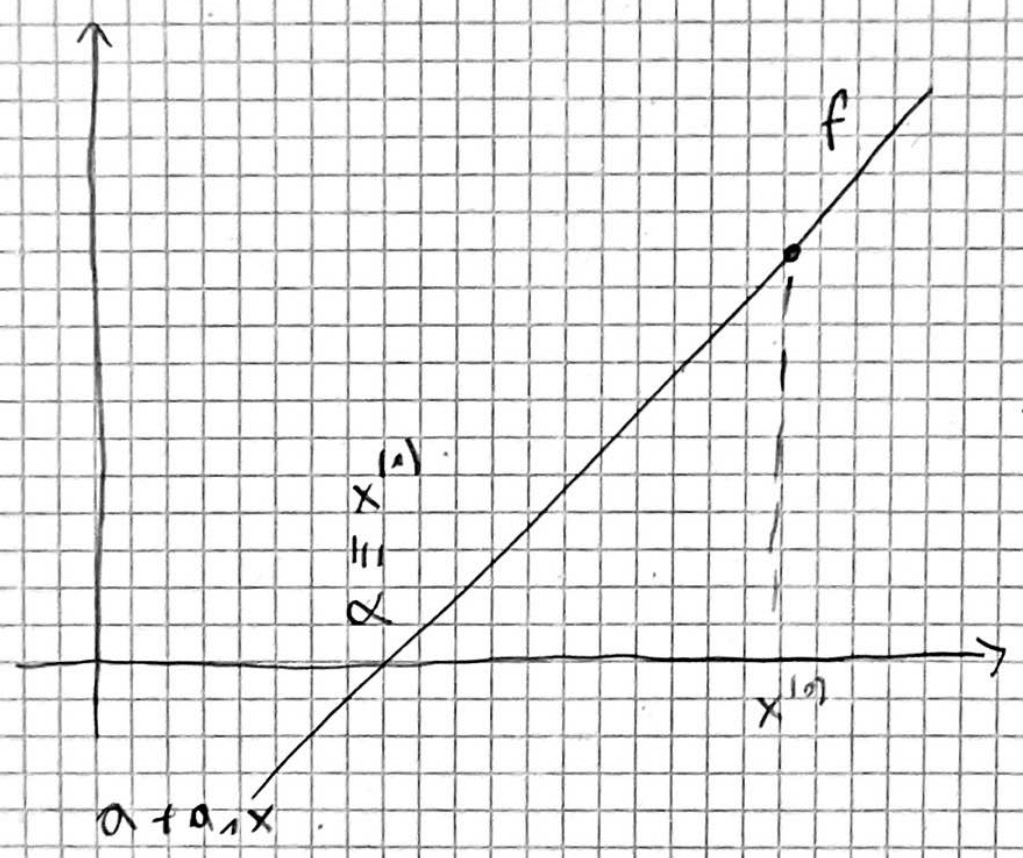
\includegraphics[width=0.5\textwidth]{images/Screenshot from 2022-09-20 22-40-18.png}}%
    \end{minipage}
\end{figure}

Analytical proof:
$$x^{(1)}=x^{(0)}-\frac{f(x^{(0)})}{f'(x^{(0)})}=x^{(0)}-\frac{
    a_0+a_1x^{(0)}
}{a_1}=-\frac{a_0}{a_1}$$

Bisection converges without initial guess, but Newton is better even though it needs an initial guess. \textbf{If initial guess not close to the zero, we do not converge}

\subsubsection{Convergence}
Two hypothesis
\begin{enumerate}[H1)]
    \item $x^{(0)}$ sufficiently close to $\alpha$. But we do not know $\alpha$, we could:
    \begin{itemize}
        \item Graphically plot it
        \item Do some steps of the bisection and use some outputs of it for Newton: \textbf{bisection-Newton: predictor-corrector}, use a weaker method then a stronger one. With bisection we know that we will converge, even if slowly, then after a desired steps (sufficiently close) we use Newton which is faster
    \end{itemize}
    \item $\alpha$ is a simple zero of $f$
    $$
    \begin{cases}
        f(\alpha)=0\\
        f'(\alpha)\neq 0
    \end{cases}
    $$
    Reminder, an $\alpha$ is a zero of order $m$ if
    $$
    \begin{cases}
        f(\alpha)=f'(\alpha)=f''(\alpha)=\cdots=f^{(m-1)}(\alpha)=0\\
        f^{(m)}(\alpha)\neq 0        
    \end{cases}
    $$
\end{enumerate}
$\mathbf{\Rightarrow}$ \textbf{Newton is convergent}

Adding a third hypothesis
\begin{enumerate}[H3)]
    \item $f\in C^2([a,b])$, we can say that the following limit holds:
    $$\lim_{k\rightarrow\infty}\frac{
        x^{(k+1)}\alpha
    }{[x^{(k)}-\alpha]^2}=
    \underlabel{\frac{f''(\alpha)}{2f'(\alpha)}}{C}$$
    In general \textbf{convergence order} equal to P if $\exists\,\,c$ independent from $k$, such that
    $$\frac{|x^{k+1}-\alpha|}{|x^k-\alpha|^P}\leq C,\,\,\forall\,\,k\geq k_0$$
    If $P=1$, linear convergence. In our case $P=2$, quadratic convergence. In general, with a higher convergence order the error reduces:
    
    $
    x^{(k)}-\alpha=10^{-2}\\
    x^{(k)}-\alpha\simeq 10^{-4}\qquad P=2\\
    x^{(k)}-\alpha\simeq 10^{-6}\qquad P=3
    $

    The constant $C$ does not have any requirement, but in some sense it is slowing the convergence (for $C=10,P=3,\text{the error }\simeq 10^{-6}*10=10^{-5}$), but for $P=1$ reduction of the error not guaranteed if $C=1$, so:
    $$P=1\rightarrow C<1$$
    In the Newton case:
    $$C=\frac{f''(\alpha)}{2f'(\alpha)}$$
\end{enumerate}
\subsubsection{Modified Newton scheme}
What if H2 does not hold, can we still use Newton? Yes, but we lose the quadratic order of the convergence.\\
If $\alpha$ is a multiple zero of $f$ (multiplicity $m$) and if $x^{(0)}$ is sufficiently close to $\alpha\Rightarrow$ Newton converges linearly ($P=1$, we lost an order of convergence)

We can use the modified Newton scheme:
$$x^{(k+1)}=x^{(k)}-m\frac{f(x^{(k)})}{f'(x^{(k)})}\qquad k\geq 0$$
Example:
$$f(x)=(x-1)\log(x)$$
$$\alpha=1$$
$$m=2$$
\begin{figure}[!ht]
    \begin{minipage}{\linewidth}
        \centering
        \makebox[\textwidth][c]{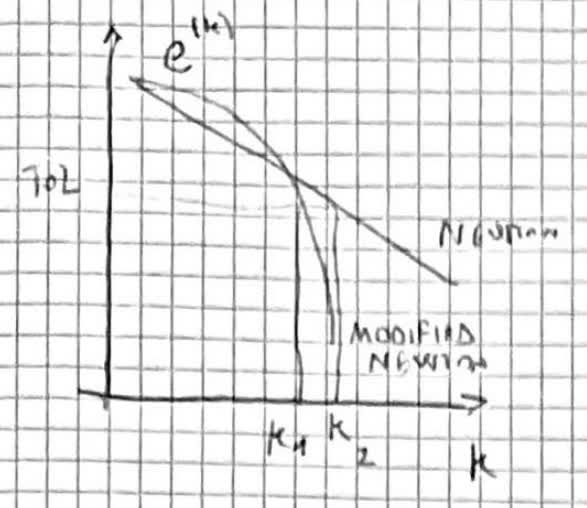
\includegraphics[width=0.6\textwidth]{images/Screenshot from 2022-09-27 18-43-43.png}}%
        %\caption{Modified Newton graph}
        %\label{BarsNielsenCrop}
    \end{minipage}
\end{figure}

\subsubsection{System of nonlinear equations, vector}
$$
\begin{cases}
    f_1(x_1,x_2,\cdots,x_n)=0\\
    f_2(x_1,x_2,\cdots,x_n)=0\\
    \vdots\\
    f_n(x_1,x_2,\cdots,x_n)=0\\
\end{cases}
$$
Example
$$
\begin{cases}
    f_1(x_1,x_2)=x_1^3+\sin x_2=0\\
    f_2(x_1,x_2)=-x_1\sqrt{x_2}+\text{tg}\left(\frac{x_2}{3x_1}\right)=0
\end{cases}
$$
We can rewrite this complex model to a more manageable form, a \textbf{vectorial way}
$$\overrightarrow{x}=[x_1,x_2,\cdots,x_n]^T$$
$$\overrightarrow{f}=[f_1(\overrightarrow{x}),f_2(\overrightarrow{x}),\cdots,f_n(\overrightarrow{x})]^T$$
$$\overrightarrow{0}=[0,\cdots,0]^T\in\mathbb{R}^n$$
So we can rewrite the system of nonlinear equations in:
$$\overrightarrow{f}(\overrightarrow{x})=\overrightarrow{0}$$
Now applying the Newton method, we jsut introduce the vectors that contain the $k$-approximation error:
$$x^{(k+1)}=x^{(k)}-\frac{f(x^{(k)})}{f'(x^{(k)})}$$
Now with
$$\overrightarrow{x}^{(k)}=\left[x_1^{(k)},x_2^{(k)},\cdots,x_n^{(k)}\right]^T\in\mathbb{R}^n$$
$$\overrightarrow{x}^{(k+1)}=\left[x_1^{(k+1)},x_2^{(k+1)},\cdots,x_n^{(k+1)}\right]^T\in\mathbb{R}^n$$
$$\overrightarrow{f}(\overrightarrow{x}^{(k)})=\left[f_1(\overrightarrow{x}^{(k)}),f_2(\overrightarrow{x}^{(k)}),\cdots,f_n(\overrightarrow{x}^{(k)})\right]^T\in\mathbb{R}^n$$
What about the derivative? Use Jacobian
$$x^{(k+1)}=x^{(k)}-\underlabel{\frac{f(x^{(k)})}{f'(x^{(k)})}}{$\delta x^{(k)}$}$$
$$f'(x^{(k)})\delta x^{(k)}=-f(x^{(k)})$$
$$\overrightarrow{x}^{(k+1)}=\overrightarrow{x}^{(k)}+\delta\overrightarrow{x}^{(k)}$$
$$?\,\,\delta\overrightarrow{x}^{(k)}=-\overrightarrow{f}(\overrightarrow{x}^{(k)})$$
The Jacobian
$$\left(J_F\right)_y=\frac{\partial f_i}{\partial x_j}\qquad i,j=1,\cdots,n$$
The question mark becomes
$$
\underlabel{J_F\left(\overrightarrow{x}^{(k)}\right)}{$\mathbb{R}^{n\times n}$}
\underlabel{\delta x^{(k)}}{$\mathbb{R}^n$}=
\underlabel{-\overrightarrow{f}(\overrightarrow{x})^{(k)}}{$\mathbb{R}^n$}
$$

\subsubsection{Bisection - Newton method}
They are predictor-corrector mtehods. Newton is conditional convergent (the initial guess bust be close to the root), while bisection is unconditional convergent: \textbf{by using bisection we are sure that the intial guess is close to the root (predictor) then use Newton as corrector}.

\subsection{Convergence order}

$$
\brackets{x^{(k)}}\simeq\alpha
$$
Convergence order equal to p if $\exists\,\,c$ independent from $k$, such that $\frac{|x^{k+1}-\alpha|}{|x^k-\alpha|^p}\leq c,\,\,\forall\,\,k\geq k_0$
\begin{itemize}
    \item \textbf{Bisection}, error no monotone, no convergence order
    \item \textbf{Newton}
    $$x^{(k+1)}=x^{(k)}-\frac{f(x^{(k)})}{f'(x^{(k)})}\qquad k\geq 0$$
    In Newton, under assumptions that:
    \begin{itemize}
        \item $f(\alpha)=0$
        \item $f'(\alpha)\neq 0$
    \end{itemize}
    $\alpha$ simple zero, we have
    \begin{itemize}
        \item Convergence order of 1 if $f\in C^1$
        \item Convergence order of 2 if $f\in C^2$
    \end{itemize}
    If $\alpha$ not simple, $f\in C^2$, $\alpha$ is a zero of order $m\,\,(f(\alpha)=0,\cdots,f^{(m-1)}(\alpha)=0,f^{(m)}(\alpha)\neq 0)$, more simply when there is a power the zero is of the order of that power.
    \item \textbf{Modified Newton method}, unlike bisection, with newton we can compute the convergence order. Can find non-simple zeros, we have a convergence order of 2 for example. We use a different update rule:
    $$x^{(k+1)}=x^{(k)}-m\frac{f(x^{(k)})}{f'(x^{(k)})}\qquad k\geq 0$$
\end{itemize}
$$e=\brackets{|x^k-\alpha|}_k$$
$$e^k=|x^k-\alpha|$$
$$\text{Convergence order = }p=\frac{
\log\left[
    \frac{e^{k+2}}{e^{k+1}}
\right]
}{
\log\left[
    \frac{e^{k+1}}{e^{k}}
\right]
}$$
\textbf{Do not mix up exponential and error, the $e^{k}$ there stands for the error vector considering index from $k$ to $end$}

\subsection{Stopping criteria/point}
$$\underlabel{|x^{(k)}-\alpha|}{$e^{(k)}$}\leq \underlabel{CS}{Error estimator}<TOL$$
$$
\left|e^{(kmin)}\right|=\left|x^{(kmin)}-\alpha\right|\leq CS=C\left|x^{(kmin+1)}-x^{(kmin)}\right|\leq TOL\,\,(e.g.=10^{-9})
$$
A constant that multiplies our error estimator $S$. If large like $10^4$ we lose 4 orders. It is called the \textbf{reliability}, if
\begin{itemize}
    \item $C=O(1)$, estimator reliable
    \item $C=O(10^s)$, not reliable
\end{itemize}
Two kinds of estimators for the error, when one not reliable, can rely on the other one
$$
S=
\begin{cases}
    x^{(k+1)}-x^{(k)}\text{ increment, if convergence this difference becomes smaller and smaller}\\
    \qquad\text{\textbf{Newton}}\\
    r^{(k)}=f(x^{(k)})\text{ residual, huge if $x^{(k)}$ far from $\alpha$, less it is, smaller is the error}\\
    \qquad\text{\textbf{Bisection}}
\end{cases}
$$

The increment one, cycle till:
$$|x^{(k+1)}-x^{(k)}|>TOL\,\,\&\&\,\,i<TOL$$

\pagebreak

\subsubsection{Reliability of the residual}
\begin{figure}[!ht]
    \begin{minipage}{\linewidth}
        \centering
        \makebox[\textwidth][c]{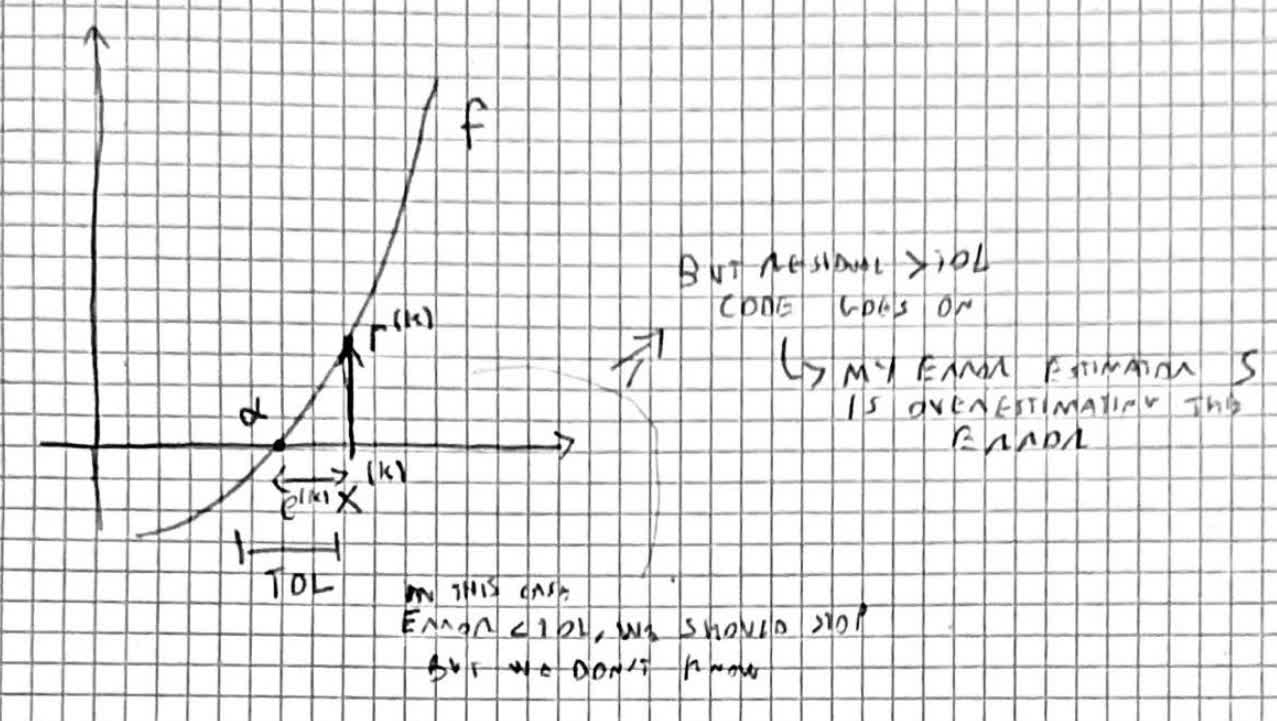
\includegraphics[width=1\textwidth]{images/Screenshot from 2022-09-27 18-43-57.png}}%
        \caption{Overestimating}
        %\label{BarsNielsenCrop}
    \end{minipage}
\end{figure}
My error estimator $S$ is overestimating the error $e^{(k)}$
$$|f'(\alpha)| >> 1$$

\begin{figure}[!ht]
    \begin{minipage}{\linewidth}
        \centering
        \makebox[\textwidth][c]{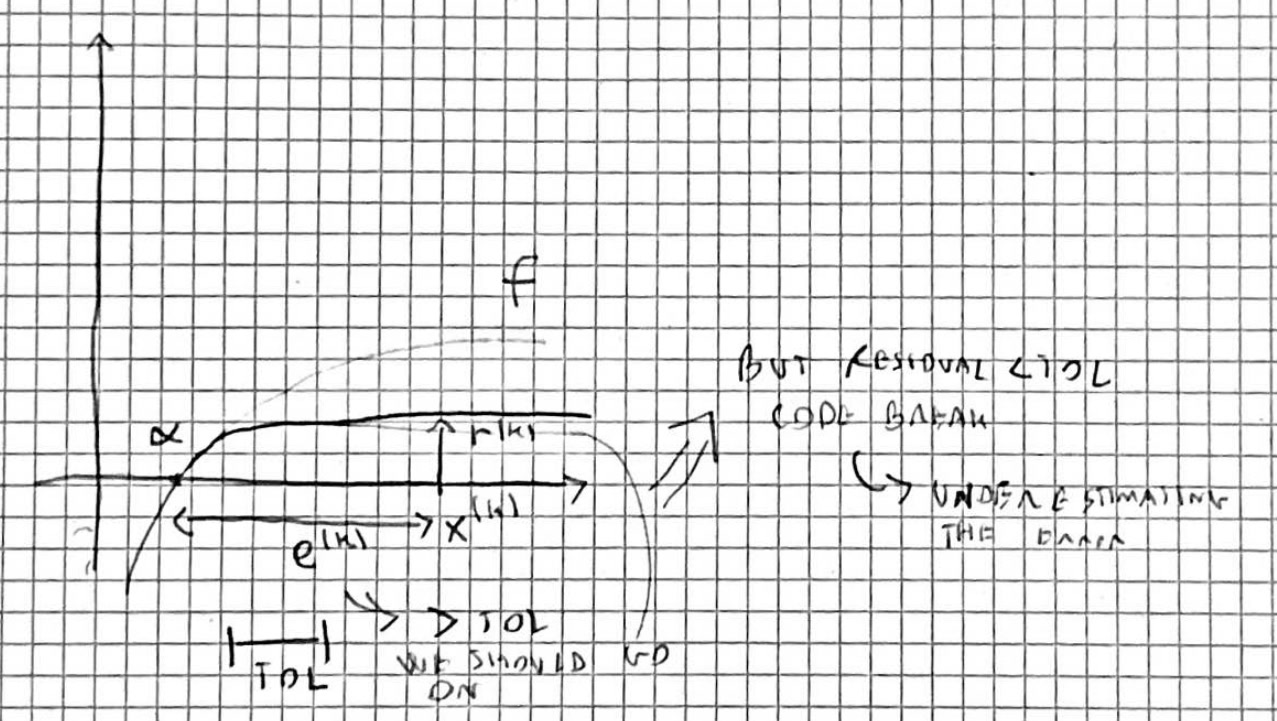
\includegraphics[width=1\textwidth]{images/Screenshot from 2022-09-27 18-44-12.png}}%
        \caption{Underestimating}
        %\label{BarsNielsenCrop}
    \end{minipage}
\end{figure}
My error estimator $S$ is underestimating the error $e^{(k)}$
$$|f'(\alpha)| << 1$$

What's better? Better when overestimating, we do a little more work, but at the end we get the better result

So this estimator is reliable when:
$$|f'(\alpha)| \simeq 1$$

\subsection{Fixed Point Method}
If we apply continuously for example the cos:

$
x^{(0)}=1\\
x^{(1)}=\cos(x^{(0)})\\
x^{(2)}=\cos(x^{(1)})\\
\vdots\\
x^{(k+1)}=\cos(x^{(k)})
$

Which means $\alpha=\cos(\alpha)$, with $\alpha$ known as \textbf{fixed point} of the function cos. In general:
$$\Phi:[a,b]\subset\mathbb{R}\rightarrow \mathbb{R}$$
$$\alpha\in\mathbb{R}\text{ fixed point $\phi(\alpha)=\alpha$}$$
Geometrically we are looking for the intersection of:
$$
\begin{cases}
    y=\phi(x)\\
    y=x\qquad\text{Bisector line}
\end{cases}
$$

\begin{figure}[!ht]
    \begin{minipage}{\linewidth}
        \centering
        \makebox[\textwidth][c]{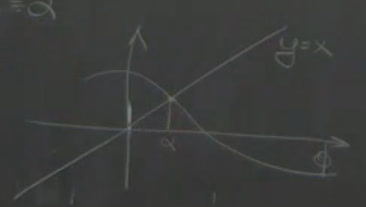
\includegraphics[width=0.8\textwidth]{images/Screenshot from 2022-10-02 16-20-18.png}}%
        %\caption{Fixed point geometric interpretation}
        %\label{BarsNielsenCrop}
    \end{minipage}
\end{figure}

\begin{itemize}
    \item Does any function has a fixed point? No, for example parallel line or exponential function, it grows fast and does not encounter the bisector line
    \item Does a function admit more fixed points? Yes, function can encounter the bisector line multiple times
\end{itemize}
How can a fixed point interest us? We can talk about a sort of duality problem:
$$
\begin{cases}
    ?\,\,\alpha\in\mathbb{R}\,\,st\,\,f(\alpha)=0\qquad\text{Our original problem of zeros}\\
    ?\,\,\alpha\in\mathbb{R}\,\,st\,\,\phi(\alpha)=\alpha\qquad\text{Fixed point problem}
\end{cases}
$$

\subsubsection{Problems correlation}
The transition:
$$
\begin{bmatrix}
    ?\,\,\alpha\in\mathbb{R}\,\,st\,\,f(\alpha)=0 & \Leftrightarrow & ?\,\,\alpha\in\mathbb{R}\,\,st\,\,\phi(\alpha)=\alpha\\
    \\
    f(x)=0 & \Leftrightarrow & \underlabel{f(x)+x}{$\phi(x)$}=x
    \\
    \\
    \Rightarrow \text{Hp: }f(\alpha)=0 & &\Leftarrow\text{Hp: }\phi(\alpha)=\alpha\\
    \text{Th: }\phi(\alpha)=\alpha & & \text{Th: }f(\alpha)=0\\
    \phi(\alpha)=\underlabel{f(\alpha)}{=0}+\alpha=\alpha & & \underlabel{\phi(\alpha)}{$=\alpha$}=f(\alpha)+\alpha=\alpha
\end{bmatrix}
$$
But the $\phi$ is not unique, we can build more and different fixed point functions (e.g. add constant multiplier), this is a \textbf{advantage}, we can pick a function that is for sure to have a fixed point

\subsubsection{The method with Newton and Bisection}
With an \textbf{iterative process}, now we try to solve
$$?\,\,\alpha\in\mathbb{R}\,\,st\,\,\phi(\alpha)=\alpha$$
With iterative method
$$x^{(k+1)}=\phi(x^{(k)})\qquad k\geq 0$$
With initial guess $x^{(0)}$. Considering the previous methods bisection and Newton, can we rewrite them as a fixed point method?
\begin{itemize}
    \item \textbf{Newton}: we can just pick a fixed point function as:
    $$\phi_N(x)=x-\frac{f(x)}{f'(x)}$$
    \item \textbf{Bisection}: no, the midpoint depends on two variables, so bisection is not an example of fixed point method
\end{itemize}

\pagebreak
\subsubsection{Convergence}
\begin{figure}[!ht]
    \begin{minipage}{\linewidth}
        \centering
        \makebox[\textwidth][c]{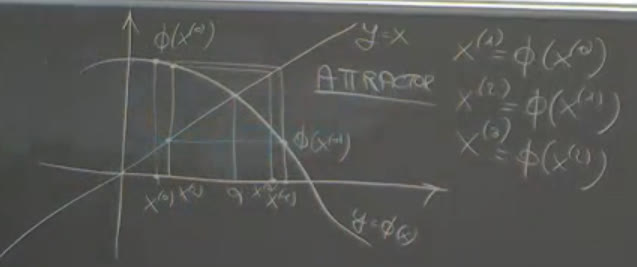
\includegraphics[width=0.8\textwidth]{images/Screenshot from 2022-10-02 17-20-18.png}}%
        \caption{Attractor}
        %\label{BarsNielsenCrop}
    \end{minipage}
\end{figure}

All even at left side, all even at right side.\\
Are we converging to $\alpha$? Yes, the iterations are moving closer and closer to $\alpha$, which is an \textbf{attractor}.

\begin{figure}[!ht]
    \begin{minipage}{\linewidth}
        \centering
        \makebox[\textwidth][c]{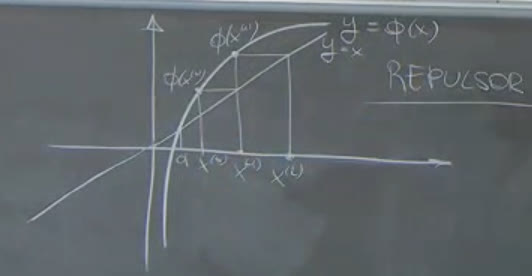
\includegraphics[width=0.8\textwidth]{images/Screenshot from 2022-10-02 17-20-20.png}}%
        \caption{Repulsor}
        %\label{BarsNielsenCrop}
    \end{minipage}
\end{figure}

In this case we are unlucky, we diverge, \textbf{repulsor}.

These are two particular cases, in total there are four: left-right convergent, left-right divergent, one direction convergent, one direction divergent.

Can we identify some features that are responsible for the convergent and divergent trend? The \textbf{value of the derivative $\phi'(\alpha)$ if less or greater than 1}

\pagebreak
\subsubsection{Global and Local Convergence Results}
$$x^{(k+1)}=\phi(x^{(k)})$$
\begin{itemize}
    \item \textbf{Global result}
    \begin{enumerate}
        \item Let $\phi\in C^0([a,b])$ and s.t. $\phi\in[a,b]\,\,\forall\,\,x\in[a,b]$\\
        \begin{figure}[!ht]
            \begin{minipage}{\linewidth}
                \centering
                \makebox[\textwidth][c]{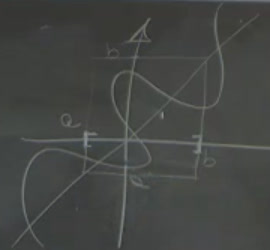
\includegraphics[width=0.4\textwidth]{images/Screenshot from 2022-10-02 17-28-19.png}}%
                %\caption{Demand 1}
                %\label{BarsNielsenCrop}
            \end{minipage}
        \end{figure}
        
        We are demading that our function $\phi$ has to take values inside that rectangle, must be limited in a certain portion of the plane.\\
        Under this hypothesis, we can prove that exists at least a fixed point $\alpha\in\,\,[a,b]$ for function $\phi$ (the example has two), so \textbf{not uniqueness of fixed point}
        \item If we in addition we assume that there exists and integer $L<1$ s.t.
        $$\left|\phi(x_1)-\phi(x_2)\right|\leq L|x_1-x_2|\,\,\forall\,\,x_1,x_2\in[a,b]$$
        (Lipschitz continuity, weaker demand w.r.t. derivability, weaker than $C^1$) then $\exists!\,\,\alpha\in[a,b]$ for $\phi$ and
        $$\brackets{x^{(k)}}\rightarrow\alpha\,\,\forall\,\,x^{(0)}\in\mathbb{R}$$
        Collection of approximations, with this assumption we get \textbf{uniqueness of fixed point and convergence of method independently from initial guess}.\\
        About the \textbf{rate of convergence of fixed point scheme with Lipschitz}, consider the error associated with $k+1$:
        $$|x^{(k+1)}-\alpha|=|\phi(x^{(k)})-\phi(\alpha)|\leq L|x^{(k)}-\alpha|$$
        $$\frac{|x^{(k+1)}-\alpha|}{|x^{(k)}-\alpha|}\leq L < 1$$
        Which means that the fixed method is convergent with order 1 (power below is 1, but actually $p\geq 1$, so \textbf{order at least 1})
    \end{enumerate}
    But this practical is not practical
    \item \textbf{Local result or Ostrowski's theorem}: let $\alpha$ be a fixed point for $\phi$ in $[a,b]$ (so we are already assuming the existence and uniqueness of $\alpha$), with $\phi\in C^1(I_\alpha)$ and $I_\alpha$ neighborhood of $\alpha$ (different from before, we here stronger assumptions than global which only required $C^0$ and Lipschitz continuity, but $C^1$ locally).\\
    Under these hypotheses, if $|\phi'(\alpha)|<1$ then $\exists\,\,\delta>0$ s.t. $\forall\,\,x^{(0)}$ with $|x^{(0)}-\alpha|<\delta$:
    $$\brackets{x^{(k)}}\rightarrow\alpha \text{ and }\lim_{k\rightarrow\infty}\frac{x^{(k+1)}-\alpha}{x^{(k)}-\alpha}=\phi'(\alpha)$$
    To summarize if:
    $$
    \begin{cases}
        |\phi'(\alpha)| < 1 \text{ convergence}\\
        |\phi'(\alpha)| > 1 \text{ divergence}\\
        |\phi'(\alpha)| = 1 \text{ we cannot say anything}\\
    \end{cases}
    $$
\end{itemize}

\subsubsection{Examples for the Local Result}
\begin{enumerate}
    \item $\phi(x)=\cos(x)$ and $\phi'(x)=-\sin(x)$
    $$|\phi'(\alpha)|=|\sin(\alpha)|<1\qquad \alpha\neq 0$$
    \item $\phi(x)=x^2-1$, we want to know if fixed point method is convergent or not: first we derive the fixed point of $\phi$:
    $$x=\phi(x)\rightarrow x^2-x-1=0$$
    $$\alpha_{1,2}=\frac{1\pm\sqrt{5}}{2}$$
    So two fixed point, now compute derivative
    $$\phi'(x)=2x\rightarrow|\phi'(\alpha)|=\left|1\pm\sqrt{5}\right|$$
    In neither cases the module is less than 1, so divergent fixed point method
    \item $\log(x)=\gamma$ with $\gamma\in\mathbb{R}$, we are demanded to approximate this function with fixed point:
    $$f(x)=0\rightarrow \underlabel{\log(x)-\gamma}{$f(x)$}=0$$
    We can use whatever method/fixed point function we like:
    \begin{enumerate}
        \item With Newton
        $$\phi_1(x)=\phi_N(x)=x-\frac{\log(x)-\gamma}{\frac{1}{x}}=x(1-\log(x)+\gamma)$$
        \item 
        $$\phi_2(x)=\log(x)-\gamma+x$$
        \item 
        $$x\log(x)-\gamma x=0\rightarrow\phi_3(x)=\frac{x\log(x)}{\gamma}$$
    \end{enumerate}
    For $\gamma=-2$, we can verify that $\phi_1$ and $\phi_3$ are ok, while for the $\phi_2$ it does not work
\end{enumerate}

\subsubsection{Fixed point method with any order of convergence}
Proposition: let us assume that the Ostrowski's theorem hypothesis are verified (\textbf{so we are in local setting}). If $\phi\in C^P(I_\alpha)$ and $\phi^{(i)}(\alpha)=0\,\,i=1,\cdots,p-1$ (derivatives till $p-1$) and $\phi^{(p)}(\alpha)\neq 0$ then $\exists\,\,\delta>0$ s.t. $\forall\,\,x^{(0)}$ with $\left|x^{(0)}-\alpha\right|<\delta$
$$
\brackets{x^{(k)}}\rightarrow\alpha\text{ and }\lim_{k\rightarrow\infty}\frac{x^{(k+1)}-\alpha}{\left[x^{(k)}-\alpha\right]^p}=\underlabel{\frac{\phi^{(p)}}{p!}}{$C$}
$$
We can guarantee the convergence of our fixed point method and compute the convergence order.

\subsubsection{Stopping criteria}
Reminder
$$
\left|e^{(kmin)}\right|=\left|x^{(kmin)}-\alpha\right|\leq CS=\left|x^{(kmin+1)}-x^{(kmin)}\right|\leq TOL\,\,(e.g.=10^{-9})
$$
Reminder: $\exists\,\,\beta_k$ between $\alpha$ and $x^{(k)}$ (min value theorem, appliable since $\phi$ is $C^1$)
$$
\alpha-x^{(k+1)}=\phi(\alpha)-\phi(x^{(k)})=\phi'(\beta_k)(\alpha-x^{(k)})
$$
So, adding and subtracting $x^{(k+1)}$:
$$
\alpha-x^{(k)}=\alpha-x^{(k+1)}+\underlabel{x^{(k+1)}-x^{(k)}}{$\delta^{(k)}$}=\phi'(\beta_k)(\alpha-x^{(k)})+\delta^{(k)}
$$
$$
\alpha-x^{(k)}=\frac{1}{1-\phi'(\beta_k)}(x^{(k+1)}-x^{(k)})
$$
For $k$ sufficiently large we can identify $x^{(k)}$ with $\alpha$ and $\beta_k$ with $\alpha$. So the error associated with the $k$ iteration is:
$$
\alpha-x^{(k)}\cong\underlabel{\frac{1}{1-\phi'(\alpha)}}{$C$}(x^{(k+1)}-x^{(k)})
$$
For $C$ as much as possible close to 1, it means that $\phi'(\alpha)$ is very small, almost zero.
$$
\phi'(\alpha)=0\rightarrow\text{convergence order of at least 2! Quadratic convergence}
$$

An \textbf{example}:
$$
f(x)=(x-1)^{(n-1)}\log(x)
$$
With one zero $\alpha=1$ with multeplicity $m$. We can prove that:
$$\phi'(\alpha)=1-\frac{1}{m}$$
Larger is $m$, closer that quantity is to 1, which means we are losing in terms of reliability ($C$ is growing to infinity).

\begin{figure}[!ht]
    \begin{minipage}{\linewidth}
        \centering
        \makebox[\textwidth][c]{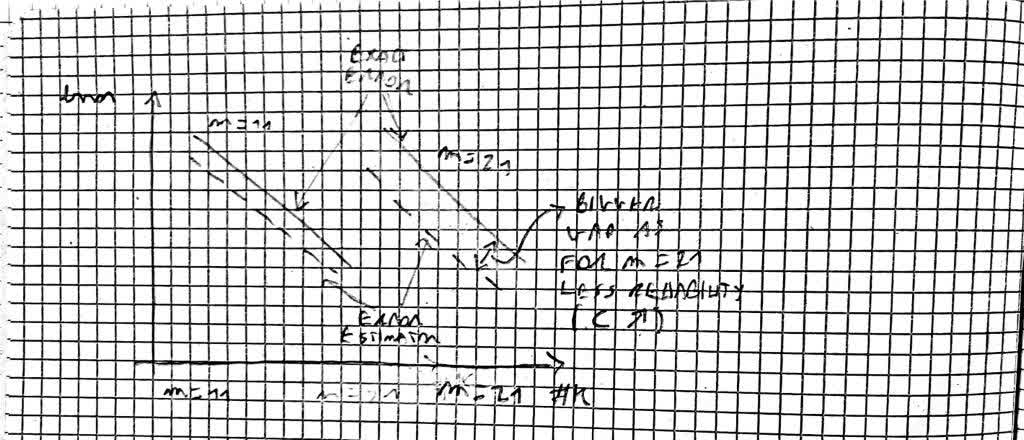
\includegraphics[width=1\textwidth]{images/Screenshot from 2022-10-04 17-28-19.png}}%
        %\caption{Trend of error and error estimator}
        %\label{BarsNielsenCrop}
    \end{minipage}
\end{figure}

A stopping criterion for fixed point: $m$ not too high.

\subsection{Consistency}
$$
x^{(k+1)}=\phi(x^{(k)})
$$
If $\alpha$ is a fixed point of $\phi$, the method is consistent
    % !TeX root = ../main.tex

\section{Systems of Linear Equations: Direct Methods}
We are talking about
\begin{LARGE}
$$
    Ax=b\Leftrightarrow\begin{cases}
        a_{11}x_1+a_{12}x_2+\cdots+a_{1n}x_n=b_1\\
        a_{21}x_1+a_{22}x_2+\cdots+a_{2n}x_n=b_2\\
        \vdots\hspace{11.5em}\vdots\\
        a_{n1}x_1+a_{n2}x_n+\cdots+a_{nn}x_n=b_n\\        
    \end{cases}
$$
$$
A\in\mathbb{R}^{n\times n}\qquad x,b\in\mathbb{R}^{n}
$$
\end{LARGE}

\subsection{Cramer Method}
Reminder:
$$
x_i=\frac{\det(A_i)}{\det(A)}\qquad i=1,\cdots,n
$$
Problem: finding the determinants computationally intensive, reminder of the Laplace rule:
$$
\det(A)=
\begin{cases}
    a_n\qquad\text{if $n=1$}\\
    \sum_{j=1}^n(-1)^{i+j}a_{ij}\Delta_{ij}\qquad\forall\,\,i\qquad\Delta_{ij}=\det(A_{ij})
\end{cases}
$$
Where $A_{ij}$ is the submatrix obtained by removing the $i$th row and $j$th column.\\On average we peform a number of operations equal to $3(n+1)!$, absolutely unfeasible, we must move to numerical counterparts/approximations.

\subsection{Numerical Approximations: Direct Methods}
We will talk about:
\begin{enumerate}[1)]
    \item Direct methods (fixed number of steps to get the solution, no notion of convergence)
    \item Iterative methods (non-ending number of steps, we will have to stop at a certain point, convergence)
\end{enumerate}
There is no better alternative, both depend on the kind of the problem

At the basis of the direct methods we will use the factorization of the matrix: \textbf{LU factorization}.

\subsubsection{LU factorization of a matrix}
Let $A$ a matrix, it can be expressed as the product of two matrices $A=LU$, where $L$ is a lower triangular matrix (elements different from zero on the main diagonal and on elements below) and $U$ is an upper triangular matrix.

Consider
$$
Ax=b\qquad A\text{ nonsingular}
$$
$$
L\underlabel{Ux}{$y$}=b
$$
The solution of the system then changes to
$$
\begin{cases}
    Ly=b\\
    Ux=y
\end{cases}
$$
Solve the upper system first, then the lower one

As the matrices are triangular (a lot of zeros, they are sparse), the systems are easier to solve! A matrix is defined as \textbf{sparse} if the number of entries different from zeros is a $O(n)$ istead of $O(n^2)$

A remark, if $A$ is nonsingular, then it follows that $L$ and $U$ are nonsingular as
$$\det(A)=\det(LU)=\det(L)\det(U)$$
Also since the \textbf{determinant of a triangular matrix is the product of the entries in the diagonal}, all elements on the diagonal are non-zero.

\subsubsection{Forward substitution method}
Assume $L$ and $U$ are given, we start from:
$$Ly=b$$
$$
\begin{bmatrix}
    l_{11} & 0 & 0\\
    l_{21} & l_{22} & 0\\
    l_{31} & l_{32} & l_{33}\\
\end{bmatrix}
\begin{bmatrix}
    y_1\\
    y_2\\
    y_3\\
\end{bmatrix}=
\begin{bmatrix}
    b_1\\
    b_2\\
    b_3\\
\end{bmatrix}
$$
$
l_{11}y_1=b_1\rightarrow y_1=\frac{b_1}{l_{11}}\qquad l_{11}\neq0\\
\\
l_{21}y_1+l_{22}y_2=b_2\rightarrow y_2=\frac{1}{l_{22}}\left[b_2-l_{21}y_1\right]\\
\\
l_{31}y_1+l_{32}y_2+l_{33}y_3=b_3\rightarrow y_3=\frac{1}{l_{33}}\left(b_3-l_{31}y_1-l_{32}y_2\right)
$

So for a generic lower triangular matrix $L$:
\begin{LARGE}
    $$
    y_1=\frac{b_1}{l_{11}}
    $$
    $$
    y_i=\frac{1}{l_{ii}}\left[b_i-\sum_{j=1}^{i-1}l_{ij}y_j\right] \qquad i=2,\cdots,n
    $$
\end{LARGE}

With a number of operations for each $i$:
\begin{itemize}
    \item 1 division for $l_{ii}$
    \item In the squares $i-1$ subtractions
    \item Each subtractions is a product, we have $i-1$ multiplications
\end{itemize}
So the total number of operations is:
$$
1+\sum_{i=2}^n(1+2i-2)=\sum_{i=1}^n(1+2i-1)=\sum_{i=1}^n1+2\sum_{i=1}^n(i-1)=n+2\frac{n(n-1)}{2}=\mathbf{n^2}
$$

\subsubsection{Backward substitution method}
Consider now the upper triangular system:
$$
Ux=b
$$
$$
\begin{bmatrix}
    u_{11} & u_{12} & u_{13}\\
    0 & u_{22} & u_{23}\\
    0 & 0 & u_{33}
\end{bmatrix}
\begin{bmatrix}
    x_1\\
    x_2\\
    x_3\\
\end{bmatrix}=
\begin{bmatrix}
    y_1\\
    y_2\\
    y_3\\
\end{bmatrix}
$$
$
u_{33}x_3=y_3\rightarrow x_3=\frac{y_3}{u_{33}}\\
\\
\cdots\rightarrow x_2=\frac{1}{u_{22}}\left[y_2-u_{23}x_3\right]\\
\\
\cdots
$

So for a generic lower upper matrix $U$:
\begin{LARGE}
    $$
    x_n=\frac{y_n}{u_{nn}}
    $$
    $$
    x_i=\frac{1}{u_{ii}}\left[y_i-\sum_{j=i+1}^{n}u_{ij}x_j\right] \qquad i=n-1,\cdots,1
    $$
\end{LARGE}

So the total number of operations is $n^2$

\subsubsection{Direct inspection}
Suppose we know the matrix, we want to find the $LU$ factorization:
$$
\begin{bmatrix}
    a_{11} & a_{12}\\
    a_{21} & a_{22}\\
\end{bmatrix}=
\underlabel{
    \begin{bmatrix}
        l_{11} & 0\\
        l_{21} & l_{22}\\
    \end{bmatrix}
}{$L$}
\underlabel{
    \begin{bmatrix}
        u_{11} & u_{12}\\
        u_{21} & 0\\
    \end{bmatrix}
}{$U$}
$$
In this case, we can write:
$$
\begin{cases}
    l_{11}u_{11}=a_{11}\\
    l_{11}u_{12}=a_{12}\\
    l_{21}u_{11}=a_{21}\\
    l_{21}u_{12}+l_{22}u_{22}=a_{22}        
\end{cases}
$$
We can see that we have 6 unknowns and 4 equations. By convetion we can assign "1" to the diagonal of the matrix $L$
$$
\underlabel{
    \begin{bmatrix}
        1 & 0\\
        l_{21} & 1\\
    \end{bmatrix}
}{$L$}
\underlabel{
    \begin{bmatrix}
        u_{11} & u_{12}\\
        u_{21} & 0\\
    \end{bmatrix}
}{$U$}
$$
So our system becomes:
$$
\begin{cases}
    u_{11}=a_{11}\\
    u_{12}=a_{12}\\
    l_{21}u_{11}=a_{21}\\
    l_{21}u_{12}+u_{22}=a_{22}        
\end{cases}
$$
From which we easily find the unknowns.

If we consider a generic matrix $N$:
$$
\underlabel{
    \begin{bmatrix}
        \ddots & & \ddots \\
        & A &\\
        \ddots & & \ddots 
    \end{bmatrix}
}{$n^2$ equations}=
\underlabel{
    \begin{bmatrix}
        \ddots & &\\
        & L &\\
        & & \ddots 
    \end{bmatrix}
}{With $\frac{n(n+1)}{2}$ unknowns}
\underlabel{
    \begin{bmatrix}
        \ddots & &\\
        & U &\\
        & & \ddots 
    \end{bmatrix}
}{With $\frac{n(n+1)}{2}$ unknowns}
$$
Globally with $n^2+n$ unknowns. Just like before, we assign "1" to the diagonal of $L$ so \#equations=\#unknowns

\subsubsection{Gaussian elimination method}
\textbf{GEM}, less computationally intensive than direct inspection. Consider the matrix
$$
A=\begin{bmatrix}
    a_{11} & a_{12} & a_{13}\\
    a_{21} & a_{22} & a_{23}\\
    a_{31} & a_{32} & a_{33}
\end{bmatrix}
$$
We assign for each entry a superindex to underline that it's the original matrix:
$$
A^{(1)}=\begin{bmatrix}
    a_{11}^{(1)} & a_{12}^{(1)} & a_{13}^{(1)}\\
    a_{21}^{(1)} & a_{22}^{(1)} & a_{23}^{(1)}\\
    a_{31}^{(1)} & a_{32}^{(1)} & a_{33}^{(1)}
\end{bmatrix}
$$
\begin{enumerate}
    \item First step is to move to the matrix $A^{(2)}$. Consider the coefficients:
    
    $
    l_{21}=\frac{a_{21}^{(1)}}{a_{11}^{(1)}}\qquad\text{pivot $a_{11}^{(1)}\neq 0$}\\
    \\
    l_{31}=\frac{a_{31}^{(1)}}{a_{11}^{(1)}}\qquad\text{pivot $a_{11}^{(1)}\neq 0$}
    $
    $$
    A^{(2)}=\begin{bmatrix}
        a_{11}^{(1)} & a_{12}^{(1)} & a_{13}^{(1)}\\
        0 & a_{22}^{(2)} & a_{23}^{(2)}\\
        0 & a_{32}^{(2)} & a_{33}^{(2)}
    \end{bmatrix}        
    $$
    Where
    \begin{itemize}
        \item $R2_{new}=R2_{old}-l_{21}R1_{old}$ and
        
        $
        a_{21}^{(2)}=a_{21}^{(1)}-l_{21}a_{11}^{(1)}=a_{21}^{(1)}-\frac{a_{21}^{(1)}}{a_{11}^{(1)}}a_{11}^{(1)}=0\\
        \\
        a_{22}^{(2)}=a_{22}^{(1)}-l_{21}a_{12}^{(1)}\\
        \\
        a_{23}^{(2)}=a_{23}^{(1)}-l_{21}a_{13}^{(1)}
        $
        \item $R3_{new}=R3_{old}-l_{31}R1_{old}$ and
        
        $
        a_{31}^{(2)}=a_{31}^{(1)}-l_{31}a_{11}^{(1)}=a_{31}^{(1)}-\frac{a_{31}^{(1)}}{a_{11}^{(1)}}a_{11}^{(1)}=0\\
        \\
        a_{32}^{(2)}=a_{32}^{(1)}-l_{31}a_{12}^{(1)}\\
        \\
        a_{33}^{(2)}=a_{33}^{(1)}-l_{31}a_{13}^{(1)}\\
        $
    \end{itemize}
    \item Similarly find $A^{(3)}$. Consider the coefficient:
    
    $
    l_{32}=\frac{a_{32}^{(2)}}{a_{22}^{(2)}}\qquad\text{pivot $a_{22}^{(2)}\neq 0$}
    $
    $$
    A^{(3)}=\begin{bmatrix}
        a_{11}^{(1)} & a_{12}^{(1)} & a_{13}^{(1)}\\
        0 & a_{22}^{(2)} & a_{23}^{(2)}\\
        0 & 0 & a_{33}^{(3)}
    \end{bmatrix}=U
    $$
    Where
    \begin{itemize}
        \item $R3_{new}=R3_{old}-l_{32}R2_{old}$ and
        
        $
        a_{32}^{(3)}=a_{32}^{(2)}-l_{32}a_{22}^{(2)}=a_{32}^{(2)}-\frac{a_{32}^{(2)}}{a_{22}^{(2)}}a_{22}^{(2)}=0\\
        \\
        a_{33}^{(3)}=a_{33}^{(2)}-l_{32}a_{23}^{(2)}
        $
    \end{itemize}
\end{enumerate}
Hence we found $U$. What about $L$? It is:
$$
\begin{bmatrix}
    1 & 0 & 0\\
    l_{21} & 1 & 0\\
    l_{31} & l_{32} & 1\\
\end{bmatrix}
$$
Let's see if $LU=A$, for example:
$$
A=A^{(1)}=\begin{bmatrix}
    1 & 2 & 1\\
    2 & 0 & -1\\
    -1 & 1 & 5
\end{bmatrix}
$$
\begin{enumerate}
    \item Step 1:
    $$
    A^{(2)}=\begin{bmatrix}
        1 & 2 & 1\\
        0 & -4 & -3\\
        0 & 3 & 6
    \end{bmatrix}
    $$
    With

    $
    l_{21}=2\\
    l_{31}=-1\\
    $
    \item Step 2:
    $$
    A^{(3)}=\begin{bmatrix}
        1 & 2 & 1\\
        0 & -4 & -3\\
        0 & 0 & \frac{15}{4}
    \end{bmatrix}=U
    $$
    With

    $
    l_{32}=-\frac{3}{4}
    $
\end{enumerate}
And $L$:
$$
L=\begin{bmatrix}
    1 & 0 & 0\\
    2 & 1 & 0\\
    -1 & -\frac{3}{4} & 1
\end{bmatrix}
$$
We check that:
$$
L\cdot U=
\begin{bmatrix}
    1 & 0 & 0\\
    2 & 1 & 0\\
    -1 & -\frac{3}{4} & 1
\end{bmatrix}
\begin{bmatrix}
    1 & 2 & 1\\
    0 & -4 & -3\\
    0 & 0 & \frac{15}{4}
\end{bmatrix}=
\begin{bmatrix}
    1 & 2 & 1\\
    2 & 0 & -1\\
    -1 & 1 & 5
\end{bmatrix}=A
$$
\textbf{What about the cost? It is CUBIC: } $\frac{2}{3}n^3$.

When we want to solve $Ax=b$ we have multiple ways:
\begin{enumerate}
    \item Using GEM and LU factorization
    \begin{itemize}
        \item GEM $\frac{2}{3}n^3$.
        \item Resolution of
        $$
        \begin{cases}
            Ly=b\\
            Ux=y
        \end{cases}
        $$
        Paying $2n^2$
    \end{itemize}
    Paying in total $\mathbf{\frac{2}{3}n^3+2n^2\sim O(n^3)}$
    \item GEM on $\left[A|b\right]$ paying $\mathbf{(>\frac{2}{3}n^3)+2n^2\sim O(n^3)}$
    \item Using $x=A^{-1}b$ paying an higher cost than the previous two methods. The inverse can be found applying GEM till:
    $$\left[A|I_n\right]\Rightarrow \left[I_n|A^{-1}\right]$$
\end{enumerate}
Consider methods 1 and 2, in which case one is the less costly than the other? When we have to solve multiple systems of the kind $Ax=c_{i\rightarrow q}$ with right side different every time: in this case the first method is better as we pay the cost of $LU$ factorization only once (so we pay $\frac{2}{3}n^3+q(2n^2)$) while with the second one we pay the whole cost every time (paying $q\left(\frac{2}{3}n^3+2n^2\right)$).\\
\textbf{This is the case of method 3}, we are solving $Ax=c_{i\rightarrow q}$   multiple times and in total we pay
$$\mathbf{\frac{2}{3}n^3+n(2n^2)=\frac{8}{3}n^3}$$

\subsubsection{Necessary and sufficient criteria for GEM}
$$
A=A^{(1)}\begin{bmatrix}
    1 & 1 & 3\\
    2 & 2 & 2\\
    3 & 6 & 4
\end{bmatrix}\rightarrow
A^{(2)}=\begin{bmatrix}
    1 & 1 & 3\\
    0 & 0 & -4\\
    0 & 3 & -5
\end{bmatrix}
$$
With $\left[l_{21}\,\,l_{31}\,\,l_{32}\right]=[2\,\,3\,\,\frac{3}{0}]$. The last pivot error! Some conditions:
\begin{itemize}
    \item \textbf{Necessary and sufficient condition}: let $A\in\mathbb{R}^{n\times n}$, then $LU$ factorization $\exists!$ \textbf{if and only if} the \textbf{principal submatrices} $A_i$ of $A$ for $i=1,\cdots,n-1$ are nonsingular. The principal submatrices are:
    $$
    A=\begin{bmatrix}
        A_1    & \vdots & \vdots & & \vdots & \\
        \cdots & A_2    & \vdots & & \vdots & \\
        \cdots & \cdots & A_3    & & \vdots & \\
        \cdots & \cdots & \cdots & \ddots & \vdots & \\
        \cdots & \cdots & \cdots & \cdots & A_{n-1}& \\
        \cdots
    \end{bmatrix}
    $$
    As $i$ goes to $n-1$, the matrix $A_n==A$ can be singular, a $LU$ exists anyway (but solution might not). This condition guarantess that a \textbf{LU factorization exists and it is unique}.

    Some examples
    \begin{itemize}
        \item Singular matrix but $LU$ factorization can be found
        $$
        A_1=\begin{bmatrix}
            1 & 2\\
            1 & 2
        \end{bmatrix}=
        \begin{bmatrix}
            1 & 0\\
            1 & 1
        \end{bmatrix}
        \begin{bmatrix}
            1 & 2\\
            0 & 0
        \end{bmatrix}
        $$
        \item We lose existence
        $$
        A_2=\begin{bmatrix}
            0 & 1\\
            1 & 0
        \end{bmatrix}=
        \begin{bmatrix}
            1 & 0\\
            l_{21} & 1
        \end{bmatrix}
        \begin{bmatrix}
            u_{11} & u_{12}\\
            0 & u_{22}
        \end{bmatrix}
        $$
        As $l_{21}u_{11}=1$ is impossible to satisfy as $u_{11}=0$
        \item We lose uniqueness
        $$
        A_3=\begin{bmatrix}
            0 & 1\\
            0 & 2
        \end{bmatrix}=
        \begin{bmatrix}
            1 & 0\\
            l_{21} & 1
        \end{bmatrix}
        \begin{bmatrix}
            u_{11} & u_{12}\\
            0 & u_{22}
        \end{bmatrix}
        $$
        As $l_{21}u_{11}=0$, always satisfyable as $u_{11}=0$
    \end{itemize}
    \item \textbf{Sufficient conditions for LU factorization existence and uniqueness}, 3 conditions that correspond to 3 families of lucky matrices
    \begin{enumerate}[1)]
        \item $A$ belongs to the family of the strictly diagonally dominant by rows matrices, which means that the element of the diagonal is dominant w.r.t. the other elements in the same row: the absolute value of diagonal element is strictly greater than sum of absolute value of other elements:
        $$
        |a_{ii}|>\sum_{j=1,j\neq i}^n |a_{ij}|\qquad i=1,\cdots,n
        $$
        An example that is not strictly diagonal by rows:
        $$
        \begin{bmatrix}
            -4 & 0 & 3\\
            1 & 2 & -4\\
            7 & -1 & 10
        \end{bmatrix}
        $$
        The second row does not satisfy the condition, something that satifies the condition would have second row as $[1\,\,-4\,\,2]$
        \item In some sense the dual family of the previous case: $A$ belongs to the family of the strictly diagonally dominant by columns matrices:
        $$
        |a_{jj}|>\sum_{i=1,i\neq j}^n |a_{ij}|\qquad j=1,\cdots,n
        $$
        Strictly dominant by columns does not mean it is also strictly dominant by rows, and viceversa
        \item $A$ belongs to the family of symmetric positive definite (spd) matrices.
        \begin{itemize}
            \item A matrix is symmetric if:
            $$
            a_{ij}=a_{ji}\qquad i,j=1,\cdots,n
            $$
            $$
            A=A^T
            $$
            \item A matrix is positive definite if:
            $$
            \forall\,\,x\neq 0\in\mathbb{R}\text{ for each vector, we compute the scalar and verify that:}
            $$
            $$
            x^TAx>0
            $$
        \end{itemize}
        But we perform an infinite number of checks, we consider the pair eigenvalues and eigenvectors:
        $$
        A\in\mathbb{R}^{n\times n}
        $$
        $$
        (\lambda,v)
        $$
        $$
        Av=\lambda v
        $$
        \begin{itemize}
            \item A matrix is symmetric if all eigenvalues are real numbers
            \item A matrix is positive definite if all eigenvalues are positve $\lambda >0$
        \end{itemize}
    \end{enumerate}
\end{itemize}

\subsubsection{LU strategies for particular matrices}
    \begin{itemize}
        \item If matrix $A$ is spd, we consider the $A=LU$, how does the two factors inherit the symmetric aspect of the original matrix? As
        $$A=LU=A^T=(LU)^T=U^TL^T$$
        One is the transpose of the other, so we compute only one factor. In matlab Cholesky, $R=chol(A)$, and the computational cost from $\frac{2n^3}{3}$ will be reduced to $\frac{n^3}{3}$.
        $$
        A=R^TR
        $$
        Also \textbf{the diagonal entries of matrix $R$ $r_{ii}>0$ will all be positve}.

        The \textbf{Cholesky decomposition}:
        $$
        H=
        \begin{cases}
            h_{11}=\sqrt{a_{11}}\\
            \\
            h_{ij}=\frac{1}{h_{jj}}\left(
                a_{ij}-\sum_{k=1}^{j-1}h_{ik}h_{jk}
            \right)\qquad j=1,\cdots,i-1\\
            \\
            h_{ii}=\sqrt{
                a_{ii}-\sum_{k=1}^{i-1}h_{ik}^2
            }
        \end{cases}
        $$
        Where
        $$H^T=R$$
        And our system becomes
        $$
        \begin{cases}
            Ax =b\\
            A=R^TR=HH^T
        \end{cases}
        \rightarrow
        R^TRx=b
        \rightarrow
        \begin{cases}
            R^Ty=b\\
            Rx=y
        \end{cases}
        =
        \begin{cases}
            Hy=b\\
            H^Tx=y
        \end{cases}
        $$
        \item Consider a 3-diagonal matrix, which has diagonal, first upper and first lower diagonals the only non-null overall, while all the others zero.
        $$
        A=\begin{bmatrix}
            \ddots & \ddots & 0 & 0 & 0\\
            \ddots & \ddots & \ddots & 0 & 0\\
            0 & \ddots & \ddots & \ddots & 0\\
            0 & 0 & \ddots & \ddots & \ddots\\
            0 & 0 & 0 & \ddots & \ddots
        \end{bmatrix}=
        \underlabel{
            \begin{bmatrix}
                1 & 0 & 0 & 0 & 0\\
                \ddots & 1 & 0 & 0 & 0\\
                0 & \ddots & 1 & 0 & 0\\
                0 & 0 & \ddots & 1 & 0\\
                0 & 0 & 0 & \ddots & 1
                \end{bmatrix}
        }{$L$ lower bi-diagonal, with main diagonal all 1's}
        \underlabel{
            \begin{bmatrix}
                \ddots & \ddots & 0 & 0 & 0\\
                0 & \ddots & \ddots & 0 & 0\\
                0 & 0 & \ddots & \ddots & 0\\
                0 & 0 & 0 & \ddots & \ddots\\
                0 & 0 & 0 & 0 & \ddots
            \end{bmatrix}
        }{$U$ upper bi-diagonal}
        $$
        To find the $LU$ factorization, consider
        $$
        A=\begin{bmatrix}
            a_1 & c_1 & 0\\
            e_2 & a_2 & c_2\\
            0 & e_3 & a_3
        \end{bmatrix}=
        \underlabel{
            \begin{bmatrix}
                1 & 0 & 0\\
                \beta_2 & 1 & 0\\
                0 & \beta_3 & 1            
            \end{bmatrix}    
        }{$L$}
        \underlabel{
            \begin{bmatrix}
                \alpha_1 & \gamma_1 & 0\\
                0 & \alpha_2 & \gamma_2\\
                0 & 0 & \alpha_3
            \end{bmatrix}
        }{$U$}
        $$
        It can be easily verified that
        
        $
        \gamma_1=c_1\qquad R1*C2\text{ first row of $L$ by second column of $U$}\\
        \gamma_2=c_2\qquad R2*C3
        $
        
        \vspace{1em}
        So we have 5 unknowns in $\beta_i$ and $\alpha_i$:
        
        $
        R1*C1\qquad\alpha_1=a_1\qquad\\
        R2*C1\qquad\beta_2\alpha_1=e_2\rightarrow\beta_2=\frac{e_2}{\alpha_1}\\
        R2*C2\qquad\beta_2c_1+\alpha_2=a_2\rightarrow\alpha_2=a_2-\beta_2c_1\\
        R3*C2\qquad\beta_3\alpha_2=e_3\rightarrow\beta_3=\frac{e_3}{\alpha_2}\\
        R3*C3\qquad\beta_3c_2+\alpha_3=a_3\rightarrow\alpha_3=a_3-\beta_3c_2        
        $

        \vspace{1em}
        So with a general $n\times n$ matrix:
        $$
        \begin{cases}
            \alpha_1=a_1\\
            \begin{cases}
                \beta_i=\frac{e_i}{\alpha_{i-1}}\\
                \alpha_i=a_i-\beta_ic_{i-1}\\
                i=2,\cdots,n                        
            \end{cases}            
        \end{cases}
        $$
        For every $\beta_i$ we pay 1 division, for every $\alpha_1$ we pay 1 multiplication and 1 difference, so in total we pay:
        $$3(n-1)$$
        Our problem is
        $$
        Ax=b\rightarrow LUx=b
        \rightarrow\begin{cases}
            Ly=b\\
            Ux=y
        \end{cases}
        $$
        \begin{itemize}
            \item The first equation:
            $$
            \begin{bmatrix}
                1 & 0 & 0\\
                \beta_2 & 1 & 0\\
                .0 & \beta_3 & 1
            \end{bmatrix}
            \begin{bmatrix}
                y_1\\
                y_2\\
                y_3
            \end{bmatrix}=
            \begin{bmatrix}
                b_1\\
                b_2\\
                b_3
            \end{bmatrix}
            $$
            From which:

            $
            y_1=b_1\\
            y_2=b_2-\beta_2y_1\\
            y_3=b_3-\beta_3y_2
            $

            \vspace{1em}
            Differently from forward substitution method:
            \begin{itemize}
                \item We don't have to subtract by a sum of elements
                \item There is no division term
            \end{itemize}
            And for a general $n\times n$ matrix:
            
            \begin{LARGE}
                $
                y_1=b_1\\
                y_i=b_i-\beta_iy_{i-1}\qquad i=2,\cdots,n
                $
            \end{LARGE}

            \vspace{1em}
            With cost of $2(n-1)$
            \item The second equation:
            $$
            \begin{bmatrix}
                \alpha_1 & c_1 & 0\\
                0 & \alpha_2 & c_2\\
                0 & 0 & \alpha_3
            \end{bmatrix}
            \begin{bmatrix}
                x_1\\
                x_2\\
                x_3
            \end{bmatrix}=
            \begin{bmatrix}
                y_1\\
                y_2\\
                y_3
            \end{bmatrix}
            $$
            From which:

            $
            x_3=\frac{y_3}{\alpha_3}\\
            x_2=\frac{1}{\alpha_2}[y_2-c_2x_3]\\
            x_1=\frac{1}{\alpha_1}[y_1-c_1x_2]
            $

            \vspace{1em}
            Differently from backward substitution method we don't have to subtract a summation term. For a general matrix:

            \begin{LARGE}
                $
                x_n=\frac{y_n}{\alpha_n}\\
                x_i=\frac{1}{\alpha_i}[y_i-c_ix_{i+1}]
                $
            \end{LARGE}

            \vspace{1em}
            With cost of $3(n-1)+1$

        \end{itemize}
        So in total we pay:
        $$
        \underlabel{3(n-1)}{factorization}+
        \underlabel{2(n-1)}{$Ly=b$}+
        \underlabel{3(n-1)+1}{$Ux=y$}=8n-7
        $$
        All this process is knows as \textbf{Thomas algorithm}
    \end{itemize}

\subsubsection{Rows swapping: pivoting}
    Consider this matrix:
    $$A=
    \begin{bmatrix}
        1&1&3\\
        2&2&2\\
        3&6&4
    \end{bmatrix}
    \rightarrow
    \begin{bmatrix}
        1&1&3\\
        0&0&-4\\
        0&3&-5
    \end{bmatrix}
    $$
    We have $a_{22}^{(2)}=0$, a pivot is nullable. Also if we verify the necessary and sufficient condition we see that the second principal matrix is singular. A solution is to swap the rows:
    $$A=
    \begin{bmatrix}
        1&1&3\\
        3&6&4\\
        2&2&2
    \end{bmatrix}
    \rightarrow
    \begin{bmatrix}
        1&1&3\\
        0&3&-5\\
        0&0&-4
    \end{bmatrix}
    $$
    The necessary and sufficient condition is satisfied now. Remember, \textbf{the matrix must be nonsingular}.
    
    \textbf{We perform the permutation when we meet the problem, otherwise we perform GEM all over again}.
    We exchange rows i with i+1 if:
    $$
    a_{ii}^{(i)}=0\,\,\&\&\,\,a_{i+1,i}^{(i)}\neq 0
    $$
    To do such swap we need to define a \textbf{permutation matix} $P$, an orthogonal matrix ($PP^T=P^TP=I$), obtained from identity matrix by swapping some rows. Premultipying it by our original metrix we perform the exchange, for example:
    $$
    PA=\begin{bmatrix}
        1 & 0 & 0\\
        0 & 0 & 1\\
        0 & 1 & 0
    \end{bmatrix}
    \begin{bmatrix}
        a_{11} & a_{12} & a_{13}\\
        a_{21} & a_{22} & a_{23}\\
        a_{31} & a_{32} & a_{33}
    \end{bmatrix}=
    \begin{bmatrix}
        a_{11} & a_{12} & a_{13}\\
        a_{31} & a_{32} & a_{33}\\
        a_{21} & a_{22} & a_{23}
    \end{bmatrix}
    $$
    \textbf{To exchange two rows, we just need to premultiply the original matrix by a permutation matrix. If we postmultiply $AP$ we swap columns instead}.

    This process is called \textbf{pivoting by rows}. So during GEM we keep track of swappings on the matrix $P$, so at the end we obtain $LU$ factorization not for $A$ but for $PA$
    $$PA=LU$$
    And the solution
    $$
    Ax=b\rightarrow PAx=Pb\rightarrow LUx=Pb
    $$
    $$
    \begin{cases}
        Ly=Pb\\
        Ux=y
    \end{cases}
    $$
    Only on the top equation we have effect of the permutation matrix.

    But what if the pivot is not null but very small?
    $$
    a_{ii}^{(i)}=2.5\cdot 10^{-4}
    $$
    At a certain point we will divide by it, amplifying the floating point error. Consider:
    $$
    A=\begin{bmatrix}
        1 &  1+0.5\cdot 10^{-6} & 3\\
        2 & 2 & 20\\
        3 & 6 & 4
    \end{bmatrix}
    $$
    The necessary and sufficient condition holds, the determinant of the second principal matrix is not zero but very colose to it, we can apply GEM. But the $LU$ factorization might not be accurate. The idea is to keep the pivot as large as possible in the GEM.
    
    In matlab we will use
    \begin{lstlisting}
        [L,U,P]=lu(A);
    \end{lstlisting}

\subsection{Accuracy}
This concerns iterative methods as well. Till now we saw that
$$
LU+pivoting\rightarrow \text{accurate $LU$ factorization $A-LU$}
$$
With $A$ nonsingular. If this factorization is accurate, is the solution to the system $Ax=b$ accurate as well? \textbf{No, an accurate $LU$ factorization does not necessarily ensure to have an accurate solution}.

Consider the Hilbert matrix:
$$
a_{ij}=\frac{1}{i+j-1}
$$
$$
\begin{bmatrix}
    1 & 1/2 & 1/3 & 1/4 & \cdots\\
    1/2 & 1/3 & 1/4 & \cdots\\
    1/3 & 1/4 & \cdots\\
    \cdots
\end{bmatrix}
$$
It is a symmetric matrix and positive definite, so spd. Let $A_n$ the Hilbert matrix of order $n$, consider the family of systems:
$$
A_nx_n=b_n\qquad b_n,x_n\,\,\in\mathbb{R}^n,\,\,A_n\,\,\in\mathbb{R}^{n\times n}
$$
The exact solution is
$$
b_n\,\,x_n=[1,1,\cdots,1]^T
$$
Consider the error:
$$
R_n=P_nA_n-L_nU_n\qquad(A)
$$
With each $n$ we associate:
$$
\max_{i,j}\left|r_{n_{ij}}\right|
$$
Consider the approximation $\tilde{x}_n$, the relative error
$$
E_n=\frac{||x_n-\tilde{x}_n||}{||x_n||}\qquad(B)
$$
With (B) is an accurate $LU$ factorization, but the result is not accurate
\begin{center}
    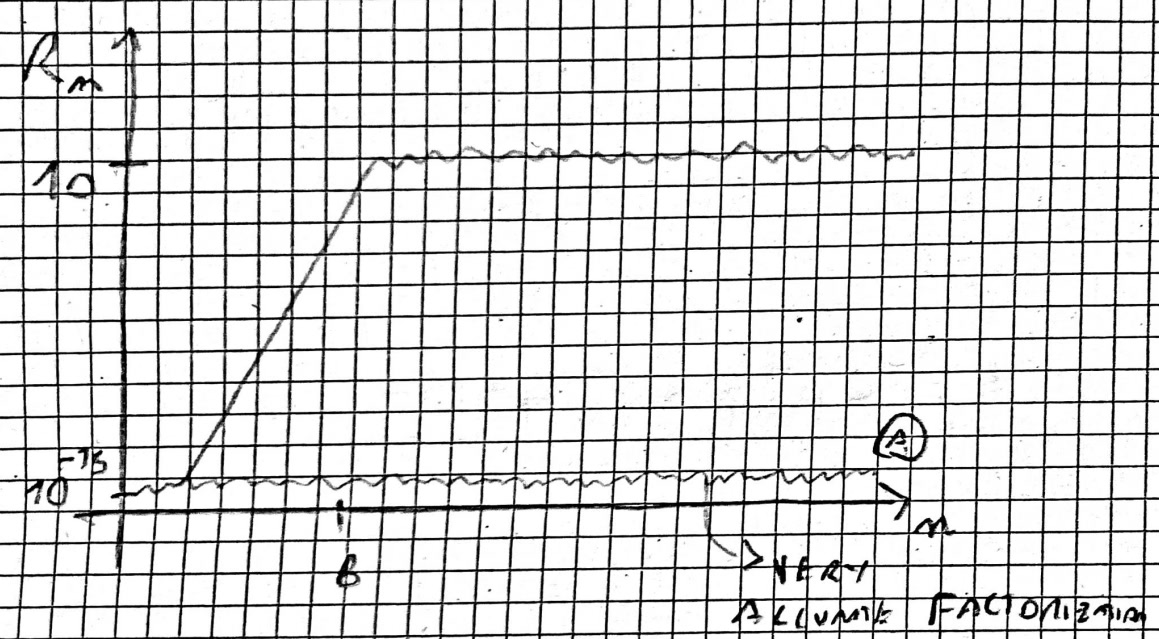
\includegraphics[width=0.8\textwidth]{images/accLU.png}
\end{center}
The reason is the problem, the Hilbert matrix is \textbf{ill positioned problem}. The method does not solve $Ax=b$, but retrieves the solution of the \textbf{perturbated system}:
$$
(A+\underlabel{\delta A}{$\mathbb{R}^{n\times n}$})(x+\delta x)=b+\underlabel{\delta b}{$\mathbb{R}^n$}
$$
$\delta b$ and $\delta A$ are perturbation on the data, matlab is computing the exact solution, but due to point floating point we will have a solution perturbation $\delta x$. We would like that for small perturbation on the data we get small perturbation on the problem (\textbf{well positioned problems}). Let the perturbated solution be
$$
\tilde{x}=x+\delta x
$$
We want to relate the two perturbations:
$$\frac{||\delta A||}{||A||}\qquad\frac{||\delta b||}{||b||}$$
We must firstly introduce some lemmas.

\subsubsection{Lemmas}
\begin{enumerate}[1)]
    \item Let $B\in\mathbb{R}^{n\times n}$ be a spd matrix. Then it holds
    $$
    \lambda_{\min}(B)\leq\frac{x^TBx}{x^Tx}\leq\lambda_{\max}(B)\qquad\forall\,\,x\neq 0\in\mathbb{R}^n
    $$
    Where $\lambda$'s are the eigenvalues.
    \item Let $A$ be a nonsingular matrix. Then $A^TA$ is spd
\end{enumerate}

\subsubsection{Perturbations relation}
Starting from $\delta A=0$, we want to relate the two perturbations:
$$\frac{||\delta A||}{||A||}\qquad\frac{||\delta b||}{||b||}$$
\begin{itemize}
    \item First step, we subtract term by term the exact system $Ax=b$ from the perturbated one $(A+0)(x+\delta x)=b+\delta b$:
    $$
    A\delta x = \delta b
    $$
    Consider the L2-norm (euclidean norm $||w||^2=w^Tw$):
    $$
    ||A\delta x||^2 = ||\delta b||^2\rightarrow
    (A\delta x)^T(A\delta x)=||\delta b||^2\rightarrow
    \delta x^TA^TA\delta x=||\delta b||^2
    $$
    From the lemma 2 $A^TA$ is spd, so we can apply lemma 1 with $B=A^TA$
    $$
    \lambda_{\min}(A^TA)\delta x^T\delta x\leq
    \delta x^TA^TA\delta x=||\delta b||^2\leq
    \lambda_{\max}(A^TA)\delta x^T\delta x
    $$
    With $\delta x^T\delta x=||\delta x||^2$. Consider only the left part of the inequality:
    $$
    \lambda_{\min}(A^TA)||\delta x||^2\leq||\delta b||^2
    $$
    $$
    ||\delta x||\leq
    \frac{
        ||\delta b||
    }{
        \sqrt{\lambda_{\min}(A^TA)}
    }
    $$
    \item As the next step consider
    $$
    ||Ax||^2=||b||^2
    $$
    Similar reasoning:
    $$
    \lambda_{\min}(A^TA)x^Tx\leq
    x^TA^Ax=(Ax)^TAx=||b||^2\leq
    \lambda_{\max}(A^TA)x^Tx
    $$
    With $x^Tx=||x||^2$. Consider only the right part of the inequality:
    $$
    ||b||\leq\sqrt{\lambda_{\max}(A^TA)}||x||
    $$
    $$
    \frac{1}{||x||}\leq\frac{\sqrt{\lambda_{\max}(A^TA)}}{||b||}
    $$
    \item We put everything together. As both inequalities are all positive quantities, we can combine them considering:
    $$
    \begin{cases}
        a\leq b\\
        c\leq d\\
    \end{cases}
    \rightarrow ab\leq cd
    $$
    \begin{LARGE}        
        $$
        \frac{||\delta x||}{||x||}\leq
        \underlabel{
            \sqrt{\frac{
                \lambda_{max}(A^TA)
            }{\lambda_{min}(A^TA)}}
        }{$K(A)\geq 1$ condition number}    
        \frac{||\delta b|}{||b||}
        $$
    \end{LARGE}

    The condition number can only amplify, a small perturbation on the data will be small as well if the condition number is almost 1 (well conditioned problem), but if the condition number is very large this relationship does not hold (ill conditioned problem, just like for Hilbert)
\end{itemize}

\subsubsection{Condition number}
$$
K(A)=||A||\cdot||A^{-1}||
$$
A norm of a matrix has 3 possible definitions
\begin{itemize}
    \item \textbf{Norm one}, maximum of the sum by columns
    \begin{center}
        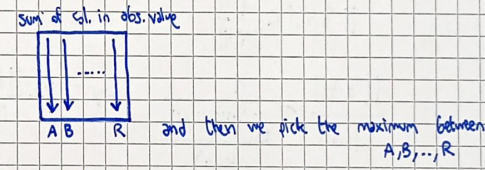
\includegraphics[width=0.8\textwidth]{images/normone.png}
    \end{center}
    $$||A||_1=\max_j\sum_{i=1}^n|a_{ij}|$$
    $$K(A)=||A||_1\cdot||A^{-1}||_1$$
    \item \textbf{Infinity norm}, first compress horizontally, then compress vertically, like dual of before
    $$||A||_\infty=\max_i\sum_{j=1}^n|a_{ij}|$$
    $$K(A)=||A||_\infty\cdot||A^{-1}||_\infty$$
    If the matrix is symmetric the infinity norm coincides with norm one
    \item \textbf{2-norm or Spectral norm}, spectrum of a matrix is the collection of the eigenvalues
    $$
    ||A||_2=\sqrt{\lambda_{\max}(A^TA)}
    $$
    From before, we found that:
    $$
    K(A)=\sqrt{\frac{
        \lambda_{max}(A^TA)
    }{\lambda_{min}(A^TA)}}=||A||_2||A^{-1}||_2
    $$
    So before we found a particular condition number:
    $$K_2(A)=||A||_2||A^{-1}||_2$$
    \begin{itemize}
        \item A special case, if $A$ is symmetric ($A=A^T$), so $A^TA=A^2$
        $$
        \lambda_{\max}(A^2)=[\lambda_{\max}(A)]^2
        $$
        And
        $$
        ||A||_2=\lambda_{\max}(A)
        $$
        $$
        K_2(A)=\frac{\lambda_{\max}(A)}{\lambda_{\min}(A)}
        $$
    \end{itemize}
\end{itemize}
In matlab $cond(A)$ for 2-norm, $condest(A_{sparse})$ for 1-norm

Now we can rewrite:
$$
\delta b = A\underlabel{(x+\delta x)}{perturbation $\tilde{x}$}-b=A\tilde{x}-b=-\tilde{r}
$$
We get the residual

\subsubsection{Perturbation on the matrix A}
What if $\delta A\neq 0$? If $||\delta A||\cdot||A^{-1}||<1$, we can:
$$
\frac{||\delta x||}{||x||}
\leq
\frac{K(A)}{1-K(A)\frac{||\delta A||}{||A||}}
\left[
    \frac{||\delta A||}{||A||}+\frac{||\delta b||}{||b||}
\right]
$$
From the hypothesis
$$
||\delta A||\cdot||A^{-1}||<1
\rightarrow
||\delta A||<\frac{1}{||A^{-1}||}
\rightarrow
\frac{||\delta A||}{||A||}<\frac{1}{||A||\cdot||A^{-1}||}
\rightarrow
K(A)\frac{||\delta A||}{||A||}<1
$$
Which means
$$
1-K(A)\frac{||\delta A||}{||A||}>0
$$
\textbf{In conclusion, before solving a problem check the condition number to see if it is ill conditioned or not. If condition number too huge problem}
    % !TeX root = ../main.tex

\section{Systems of Linear Equations: Iterative Methods}

\subsection{Iterative methods}
    We start from an initial guess $x^{(0)}\in\mathbb{R}^n$, that enters a black box that gives a $x^{(1)}$, and so on
    $$
    \Brackets{x^{(k)}}\qquad x^{(k)}\simeq x\qquad x^{(k)}\in\mathbb{R}^n
    $$

    \subsubsection{Convergence}
    we will talk about convergence again
    $$
    \lim_{k\rightarrow\infty}x^{(k)}=x
    $$
    Or alternatively express convergence in terms of error
    $$
    \begin{cases}
        e^{(k)}=x-x^{(k)}\\
        \lim_{k\rightarrow\infty}e^{(k)}=0
    \end{cases}
    $$
    \subsubsection{Consistency}
    In iterative methods we will always talk about \textbf{convergence, consistency and stability}.

    Consistency:
    $$
    x=Bx+g
    $$
    With $B$ matrix that depends on $A$ and $g$ vector that depends on $A$ and $B$
    $$
    B=B(A)\qquad g=g(A,b)
    $$
    We follow the recursive definition to create a new iteration:
    $$
    x^{(k+1)}=Bx^{(k)}+g\qquad B\in\mathbb{R}^{n\times n}\qquad g\in\mathbb{R}^n
    $$
    Consistency means that the equality has to hold w.r.t. the exact solution. Notice that $g$ depends on $A$ as:

    $
    x=Bx+g\\
    (x-Bx)=g\\
    (I-B)x=g\\
    (I-B)A^{-1}b=g
    $

    \subsubsection{Convergence analysis}
    Subtract term by term
    $$
    x^{(k+1)}=Bx^{(k)}+g\qquad -\qquad x=Bx+g
    $$
    $$
    \underlabel{x-x^{(k)}}{$e^{(k+1)}$}=\underlabel{B(x-x^{(k)})}{$e^{(k)}$}
    $$
    $$
    e^{(k+1)}=Be^{(k)}
    $$
    Compatibility of vector norms says that:
    $$
    ||e^{(k+1)}||=||Be^{(k)}||\leq ||B||_2\,\,||e^{(k)}||
    $$
    Use this inequality for convergence analysis
    $$
    ||e^{(k)}||\leq ||B||_2\,\,||e^{(k-1)}||
    \leq
    ||B||_2^2\,\,||e^{(k-2)}||
    \leq
    \cdots
    \leq
    ||B||_2^k\,\,||e^{(0)}||
    $$
    Where the following quantity is called \textbf{spectral radius}
    $$
    ||B||_2^k=[\rho(B)]^k
    $$
    Spectral radius is the maximum of the eigenvalue of the matrix taken in absolute value (in matlab $max(abs(eig(A)))$). A reminder, the 2-norm:
    $$
    ||B||_2=\sqrt{\lambda_{max}(B^TB)}
    $$
    And if $B$ is spd (eigenvalues are real positive)
    $$||B||_2=\lambda_{max}(B)$$
    Which means we are comparing $\lambda_{max}$ with itself, as in this case it is both spectral radius and 2-norm of the matrix! (\textbf{only if spd})

    To summarize:
    \begin{LARGE}
        $$
        ||e^{(k)}||\leq\left[\rho(B)\right]^k||e^{(0)}||
        $$
    \end{LARGE}
    And for convergence, the spectral radius must be less to 1
    $$
    \begin{cases}
        \rho(B)<1\\
        \lim_{k\rightarrow\infty}\left[\rho(B)\right]^k||e^{(0)}||=0
    \end{cases}
    $$
    Attention, we \textbf{assumed that the method is consistent, make sure that the method is consistent}

    This inequality represents a \textbf{necessary and sufficient condition for convergence}: let us consider the iterative scheme given by $x^{(k+1)}=Bx^{(k)}+g$ and let us assume that such a scheme is \textbf{consistent}, then the scheme turns out to be convergent independently of the initial guess, $\forall\,\,x^{(0)}\in\mathbb{R}^n$ \textbf{if and only if} $\rho(B)<1$

    A scheme to be convergent, we must check consistency and spectral radius. If one of these does not hold, the method is not convergent.

    Additionally, the smaller $\rho(B)$, the quicker the convergence.

    We can also rewrite the inequality and get
    $$
    \frac{||e^{(k)}||}{||e^{(0)}||}\leq
    \left[\rho(B)\right]^k
    \leq
    TOL
    $$
    To find $k$=minimum number of iterations

\subsection{Richardson schemes}
    We have to introduce
    $$
    P\in\mathbb{R}^{n\times n}\qquad\text{nonsingular matrix (preconditioner)}
    $$
    $$
    \alpha_k\neq 0\in\mathbb{R}^{n}
    $$
    We rewrite the original system ($Ax=b$) to
    $$
    \alpha_kAx=\alpha_kb
    $$
    And rewrite matrix $A$ with splitting
    $$
    \alpha_kA=P-(P-\alpha_kA)
    $$
    So:
    $$
    P-(P-\alpha_kA)x=\alpha_kb
    $$
    $$
    Px=\alpha_kb+(P-\alpha_kA)x
    $$
    We arbitrary choose the left side associated to $k+1$ and the right side associated to $k$:
    $$
    Px^{(k+1)}=\alpha_kb+(P-\alpha_kA)x^{(k)}
    $$
    Notice, by repliacing $x^{(k)}$ with exact solution, we get consistency: \textbf{all the Richardson schemes are consistent by construction, so no need to check it, but we have to point it out!}
    We want to reach:
    $$
    x^{(k+1)}=Bx^{(k)}+g
    $$
    Multiplying by $P^{-1}$ we will obtain:
    $$
    x^{(k+1)}=
    \underlabel{\alpha_kP^{-1}b}{$g_{\alpha_k}$}+
    \underlabel{\left(
        I-\alpha_kP^{-1}A
    \right)}{$B_{\alpha_k}$}x^{(k)}
    $$
    At this point we distinguish Richardson schemes to:
    \begin{itemize}
        \item Stationary, if $\alpha_k=\alpha$, which means it never changes at every iteration, a bad choice of $\alpha$ may hinders convergence, it must be in suitable range
        \item Dynamic if $\alpha_k$ changes at each iteration. The parameter can be tuned, it is better, but it's more computational intensive/demanding
    \end{itemize}
    $\alpha$ is the learning rate, accelerates convergence.
    Develop it:
    $$
    x^{(k+1)}=
    \alpha_kP^{-1}(
        \underlabel{
            b-Ax^{(k)}
        }{$r^{(k)}$ $k$th-residual}
    )+x^{(k)}
    $$
    We can interpret it as "next iteration=previous+correction"
    $$
    x^{(k+1)}=x^{(k)}+\alpha_kz^{(k)}
    $$
    Where this value is the \textbf{preconditioned residual}
    $$
    z^{(k)}=P^{-1}r^{(k)}
    $$
    To compute the $z^{(k)}$ just solve
    $$
    Pz^{(k)}=r^{(k)}\leftrightarrow Ax=b
    $$
    Notice that $P$ is nonsingular, and it is \textbf{arbitrarily chosen}, so we choose a diagonal, 3 diagonal or triangular matrix. Also as $P$ is always the same, use $LU$ factorization just once! We save a lot of computations!

\subsection{Stationary Richardson Schemes}
    \subsubsection{Jacobi and Gauss-Seidel methods}
    \begin{itemize}
        \item \textbf{Jacobi}, we start from an example
        $$
        \begin{cases}
            a_{11}x_1+a_{12}x_2+a_{13}x_3=b_1\\
            a_{21}x_1+a_{22}x_2+a_{23}x_3=b_2\\
            a_{31}x_1+a_{32}x_2+a_{33}x_3=b_3
        \end{cases}
        $$
        For $a_{11}\neq 0$
        $$
        \begin{cases}
            x_1=\frac{1}{a_{11}}\left[b_1-a_{12}x_2-a_{13}x_3\right]\\
            x_2=\frac{1}{a_{22}}\left[b_2-a_{21}x_1-a_{23}x_3\right]\\
            x_3=\frac{1}{a_{33}}\left[b_3-a_{31}x_1-a_{32}x_2\right]
        \end{cases}
        $$
        So far no approximation, consider
        $$
        \begin{cases}
            x_1^{(k+1)}=\frac{1}{a_{11}}\left[b_1-a_{12}x_2^{(k)}-a_{13}x_3^{(k)}\right]\\
            \\
            x_2^{(k+1)}=\frac{1}{a_{22}}\left[b_2-a_{21}x_1^{(k)}-a_{23}x_3^{(k)}\right]\\
            \\
            x_3^{(k+1)}=\frac{1}{a_{33}}\left[b_3-a_{31}x_1^{(k)}-a_{32}x_2^{(k)}\right]
        \end{cases}
        $$
        Then the generic case
        \begin{LARGE}
            $$
            x_i^{(k+1)}=\frac{1}{a_{ii}}\left[
                b_i-\sum_{j=1,j\neq i}^n a_{ij}x_j^{(k)}
            \right]
            $$
            $$
            i=1,\cdots,n\qquad a_{ii}\neq 0
            $$
        \end{LARGE}
        This method \textbf{can be parallelized}, each variable $k+1$ depends only on variables at step $k$, strength point
        \item \textbf{Gauss-Seidel}, says to use the variables at the same step, it should converge/perform faster, but not guaranteed
        \begin{LARGE}
            $$
            x_i^{(k+1)}=\frac{1}{a_{ii}}
            \left[
                b_i
                -\sum_{j=1}^{i-1} a_{ij}x_j^{(k+1)}
                -\sum_{j=i+1}^n a_{ij}x_j^{(k)}
            \right]
            $$
            $$
            i=1,\cdots,n\qquad a_{ii}\neq 0
            $$
        \end{LARGE}
        \textbf{Cannot be parallelized}
    \end{itemize}
    We now rewrite the schemes so we can reach Richardson-like form
    \begin{LARGE}
        $$
        x^{(k+1)}=
        \underlabel{\alpha_kP^{-1}b}{$g_{\alpha_k}$}+
        \underlabel{\left(
            I-\alpha_kP^{-1}A
            \right)}{$B_{\alpha_k}$}x^{(k)}
        $$
    \end{LARGE}
    \begin{itemize}
        \item \textbf{Jacobi}
        $$
        x_i^{(k+1)}=\frac{1}{a_{ii}}\left[
            b_i-\sum_{j=1,j\neq i}^n a_{ij}x_j^{(k)}
        \right]
        $$
        $$
        D=\begin{bmatrix}
            a_{11} & 0 & 0\\
            0 & \ddots & 0\\
            0 & 0 & a_{nn}\\
        \end{bmatrix}
        $$
        $$
        \overrightarrow{x}^{(k)}=\left[x_1^{(k)},x_2^{(k)},\cdots,x_n^{(k)}\right]^T
        $$
        $$
        \overrightarrow{x}^{(k+1)}=\left[x_1^{(k+1)},x_2^{(k+1)},\cdots,x_n^{(k+1)}\right]^T
        $$
        $$
        b=\left[b_1,\cdots,b_n\right]^T
        $$
        So:
        $$
        Dx^{(k+1)}=b-(A-D)x^{(k)}
        $$
        $$
        x^{(k+1)}=x^{(k)}+D^{-1}(b-Ax^{(k)})
        $$
        \begin{LARGE}
            $$
            \begin{cases}
                x^{(k+1)}=x^{(k)}+1\cdot D^{-1}r^{(k)}\\
                \alpha_{k_J}=1,P_J=D
            \end{cases}
            $$
            $$
            x^{(k+1)}=\underlabel{(I-D^{-1}A)}{
                $B_J$
            }x^{(k)}+\underlabel{D^{-1}b}{
                $g_J$
            }
            $$
        \end{LARGE}

        \item \textbf{Gauss-Seidel}
        $$
        x_i^{(k+1)}=\frac{1}{a_{ii}}
        \left[
            b_i
            -\sum_{j=1}^{i-1} a_{ij}x_j^{(k+1)}
            -\sum_{j=i+1}^n a_{ij}x_j^{(k)}
        \right]
        $$
        $$
        A=\begin{bmatrix}
            \ddots & & A-D+E\\
            & D\\
            -E & & \ddots
        \end{bmatrix}
        $$
        Where matrix $E$ is strictly lower-triangular. Similar manipulations from before, we will get
        $$
        x^{(k+1)}=x^{(k)}+(D-E)^{-1}(b-Ax^{(k)})
        $$
        \begin{LARGE}
            $$
            \begin{cases}
                x^{(k+1)}=x^{(k)}+(D-E)^{-1}r^{(k)}\\
                \alpha_{k_{GS}}=1,P_{GS}=(D-E)
            \end{cases}
            $$
            $$
            x^{(k+1)}=\underlabel{(I-(D-E)^{-1}A)}{$B_{GS}$}x^{(k)}+
            \underlabel{(D-E)^{-1}b}{$g_{GS}$}
            $$
        \end{LARGE}
    \end{itemize}
    \textbf{Both stationary, so parameter $\alpha$ not used to accelerate convergence, as it is constant}.

    \subsubsection{Convergence for Jacobi and Gauss-Seidel}
    For Richardson schemes $x^{(k+1)}=Bx^{(k)}+g$, the requirements were for consistency and spectral radius $\rho(B)<1$ (necessary and sufficient). The consistency property for Richardson schemes is automatically guaranteed.

    Additionally, we have other sufficient conditions
    \begin{itemize}
        \item \textbf{Jacobi}
        \begin{itemize}
            \item Necessary condition: $\rho(B_J)<1$
            \item Sufficient conditions (attention, referred to matrix \textbf{A}):
            \begin{enumerate}
                \item If A is strictly diagonally dominant by rows
                \item If A is strictly diagonally dominant by columns
            \end{enumerate}
        \end{itemize}
        \item \textbf{Gauss-Seidel}
        \begin{itemize}
            \item Necessary condition: $\rho(B_{GS})<1$
            \item Sufficient conditions (attention, referred to matrix \textbf{A}):
            \begin{enumerate}
                \item If A is strictly diagonally dominant by rows
                \item If A is strictly diagonally dominant by columns
                \item If A is spd
            \end{enumerate}
        \end{itemize}
    \end{itemize}
    We said that Gauss-Seidel does not necessarily outperforms Jacobi. Let $A\in\mathbb{R}^{n\times n}$ nonsingular, tridiagonal, with all $a_{ii}\neq 0$: both Jacobi and Gauss-Seidel are convergent or are divergent (they cannot be "discordant") and if they both are convergent
    $$
    \rho(B_{GS})=\left[\rho(B_J)\right]^2
    $$
    The rate of convergent is determined by the spectral radius, which means GS converges faster, more specifically
    $$
    \rho(B_J)=\frac{1}{4}\rightarrow \left(
        \frac{1}{4}
    \right)\leq \epsilon
    \rightarrow k\geq \log_4\left(\frac{1}{\epsilon}\right)
    $$
    $$
    \rho(B_{GS})=\frac{1}{4^2}\rightarrow \left(
        \frac{1}{4^2}
    \right)\leq \epsilon
    \rightarrow 2k\geq \log_4\left(\frac{1}{\epsilon}\right)
    \rightarrow k\geq \frac{1}{2}\log_4\left(\frac{1}{\epsilon}\right)
    $$
    $$
    \text{\#iterations}_{GS}\simeq
    \frac{\text{\#iterations}_{J}}{2}
    $$

    \subsubsection{Optimal acceleration parameter for stationary schemes}
    Let $A$ and $P$ be \textbf{spd matrices}. Then, the stationary Richardson scheme is convergent $ \forall\,\,x^{(0)}\in\mathbb{R}^{n\times n}$ if and only if (necessary and sufficient)
    $$
    0<\alpha<\frac{2}{\lambda_{max}(P^{-1}A)}
    $$
    Moreover
    $$
    \alpha_{opt}=\frac{2}{\lambda_{\max}(P^{-1}A)+\lambda_{\min}(P^{-1}A)}
    $$
    Finally
    $$
    \underlabel{||e^{(k)}||_A}{$x-x^{(k)}$}\leq
    \underlabel{
        \left(
            \frac{
                K(P^{-1}A)-1
            }{
                K(P^{-1}A)+1
            }
        \right)^k
    }{
        $<1$
    }||e^{(0)}||_A
    \qquad k\geq 0
    $$
    With $K$ the condition number and $||e||_A$ the energy norm:
    $$
    ||w||_A=\sqrt{w^TAw}\qquad w\leq\mathbb{R}^n
    $$
    A proof for the necessary and sufficient condition:
    \begin{itemize}
        \item Prove that
        $$
        0<\alpha<\frac{2}{\lambda_{max}(P^{-1}A)}
        $$
        Consider $B_\alpha=I-\alpha P^{-1}A$, let $\lambda_i$ eigenvalues of $P^{-1}A$ such that $$\lambda_1\geq\lambda_2\geq\lambda_3\geq\cdots\geq\lambda_n\geq 0$$
        And let the generic eigenvalue of $B_\alpha$:
        $$
        1-\alpha\lambda_i
        $$
        For convergence consistency holds since it is a Richardson scheme and $\rho(B)<1$ must hold as well, which means:
        $$
        |1-\alpha\lambda_i|<1\Rightarrow
        -1<1-\alpha\lambda_i<1\Rightarrow
        \begin{cases}
            1-\alpha\lambda_i<1\\
            1-\alpha\lambda_i>-1
        \end{cases}
        $$
        The first condition is true for $\alpha >0$, aboud the second we will get $\alpha<\frac{2}{\lambda_i}\,\,\forall i$ which will result in:
        $$
        \frac{2}{\lambda_1}\leq
        \frac{2}{\lambda_2}\leq
        \cdots\leq
        \frac{2}{\lambda_n}\leq
        \Rightarrow \alpha<\frac{2}{\lambda_1}=\frac{2}{\lambda_{max}(P^{-1}A)}
        $$
        \item Prove that $\alpha_{opt}$ is that quantity. Consider a matrix $A\in\mathbb{R}^{3\times 3}$ with $\lambda_1>\lambda_2>\lambda_3$. Remind that 
        $$
        B_\alpha=I-\alpha P^{-1}A
        $$
        $$
        |1-\alpha\lambda_1|\qquad
        |1-\alpha\lambda_2|\qquad
        |1-\alpha\lambda_3|
        $$
        Plotting them w.r.t. $\alpha$:
        \begin{center}
            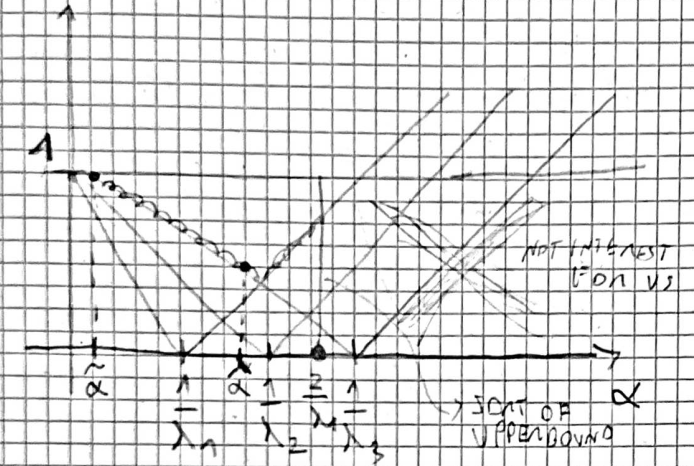
\includegraphics[width=0.9\textwidth]{images/20221118-1.png}
        \end{center}
        Analyzing those 3 plots we can understand why the optimal value is that: we are searching for $\alpha_{opt}$ such that the method is as fast as possible. A method is quicker than the other if its spectral radius is smaller than the second, which means we are finding the value for $\alpha$ such as that the maximum eigenvalue (which is related to the spectral radius) is as small as possible.\\
        On the graph we draw a vertical line in a $\tilde{\alpha}$ which will meet the 3 functions: we will get 3 eigenvalues, we consider the maximum.\\
        Observing the plot, we can see that the maximum eigenvalue is on the branches highlighted, and the $\alpha$ that minimizes the maximum eigenvalue is given by the intersection of the two branches
        $$
        \underlabel{
            1-\alpha\lambda_3
        }{Positive branch}=
        \underlabel{
            \alpha\lambda_1-1
        }{Negative branch}
        \Rightarrow
        \alpha_{opt}=\frac{2}{\lambda_1+\lambda_3}
        $$
        Which is exactly
        $$
        \alpha_{opt}=\frac{2}{\lambda_{\max}(P^{-1}A)+\lambda_{\min}(P^{-1}A)}
        $$
        About the maximum rate of convergence, the spectral radius (with $\lambda_n$ the minimum):
        $$
        \rho(B_{\alpha_{opt}})=1-\alpha_{opt}\lambda_n=
        1-\frac{2\lambda_n}{\lambda_1+\lambda_n}=
        \frac{\lambda_1-\lambda_n}{\lambda_1+\lambda_n}
        $$
        \item Prove that
        $$
        \underlabel{||e^{(k)}||_A}{$x-x^{(k)}$}\leq
        \underlabel{
            \left(
                \frac{
                    K(P^{-1}A)-1
                }{
                    K(P^{-1}A)+1
                }
            \right)^k
        }{
            $<1$
        }||e^{(0)}||_A
        \qquad k\geq 0
        $$
        With $K$ the condition number and $||e||_A$ the energy norm:
        $$
        ||w||_A=\sqrt{w^TAw}\qquad w\leq\mathbb{R}^n
        $$
        We said that the preconditioner matrix $P$ is:
        \begin{itemize}
            \item Nonsingular
            \item Easy to solve, as we have to sovle $Pz^{(k)}=r^{(k)}$
            \item \textbf{Additional condition}, $K(P^{-1}A)$ small
        \end{itemize}
    \end{itemize}

\subsection{Dynamic Richardson Scheme: preconditioned gradient methods}
    If $A$ and $P$ are spd matrices, the dynamic Richardson scheme is convergent \underline{if} (sufficient)
    $$
    \alpha_{k,opt}=\frac{
        \left[z^{(k)}\right]^Tr^{(k)}
    }{
        \left[z^{(k)}\right]^TAz^{(k)}
    }\qquad\forall\,\,k\geq 0,\,\,z^{(k)}=P^{-1}r^{(k)}
    $$
    \textbf{We directly have optimal value for $\alpha$, this method is called preconditioned gradient method}. Moreover, we can exactly prove the same inequality
    $$
    \underlabel{||e^{(k)}||_A}{$x-x^{(k)}$}\leq
    \underlabel{
        \left(
            \frac{
                K(P^{-1}A)-1
            }{
                K(P^{-1}A)+1
            }
        \right)^k
    }{
        $<1$
    }||e^{(0)}||_A
    \qquad k\geq 0
    $$
    Remark: for $P=I$, our optimal recipe for $\alpha$ becomes:
    $$
    \alpha_{k,opt}=\frac{
        \left[r^{(k)}\right]^Tr^{(k)}
    }{
        \left[r^{(k)}\right]^TAr^{(k)}
    }\qquad\forall\,\,k\geq 0,\,\,z^{(k)}=P^{-1}r^{(k)}
    $$
    \textbf{Gradient method}.
    \subsubsection{The algorithm}
    The algorithm has 4 steps
    \begin{center}
        \begin{lstlisting}[language=Matlab, escapeinside=`']
% set intial guess, we can also define associated initial residual
`$x^{(\phi)}\in\mathbb{R}^n\qquad r^{(\phi)}=b-Ax^{(\phi)}$'
for k=0,1,...
    if `$P=I$'
        % got to step 2, 3 steps algorithm in this case
    else
        `1) $Pz^{(k)}=r^{(k)}$'
    `2) $\alpha_{k,opt}=\frac{
        \left[z^{(k)}\right]^Tr^{(k)}
    }{
        \left[z^{(k)}\right]^TAz^{(k)}
    }$'
    `3) $x^{(k+1)}=x^{(k)}+\alpha_{opt,k}z^{(k)}$'
    `4) $r^{(k+1)}=r^{(k)}-\alpha_{opt,k}Az^{(k)}$'
        \end{lstlisting}
    \end{center}
    If stationary, step 2) outside the for cycle
    \begin{center}
        \begin{lstlisting}[language=Matlab, escapeinside=`']
% set intial guess, we can also define associated initial residual
`$x^{(\phi)}\in\mathbb{R}^n\qquad r^{(\phi)}=b-Ax^{(\phi)}$'
`$\alpha_{opt}=...$'
for k=0,1,...
    if `$P=I$'
        % got to step 3, 2 steps algorithm in this case
    else
        `1) $Pz^{(k)}=r^{(k)}$'
    `3) $x^{(k+1)}=x^{(k)}+\alpha_{opt}z^{(k)}$'
    `4) $r^{(k+1)}=r^{(k)}-\alpha_{opt}Az^{(k)}$'
        \end{lstlisting}
    \end{center}
    \subsubsection{Stationary and dynamic: which one is the best}
    Now that we have found the optimal acceleration parameters $\alpha_{opt}$ for both stationary and dynamic cases, which one is better? For stationary we have to find the eigenvalues, but if the matrix is very big this is too demanding, though there are methods to cope with this.

    It is a good idea to prefer dynamic scheme, as in the definition of the acceleration parameter we are using all parameters that are required to be computed for the solution of the system (in the stationary to find the eigenvalues we have to use other parameters unrelated and useless for the solution of our original problem).

    An example
    $$
    \begin{cases}
        2x_1+x_2=1\\
        x_1=3x_2=0
    \end{cases}
    $$
    \begin{center}
        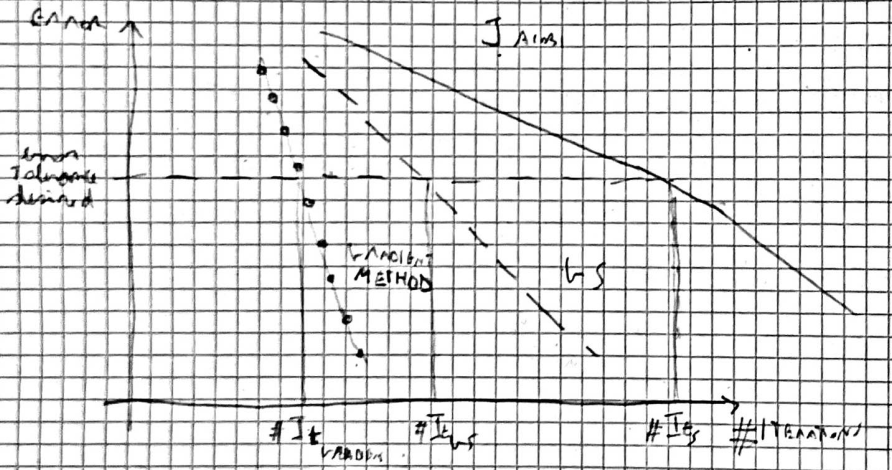
\includegraphics[width=1\textwidth]{images/20221118-2.png}
    \end{center}

    \subsubsection{Proof for the optimal acceleration parameter}
    If $A$ is spd, the solution to our system is: $Ax=b\Leftrightarrow$ equivalent to minimize the quadratic form
    $$Q(x)=\frac{1}{2}x^TAx-x^Tb$$
    as minimizing this quadratic form is solving the gradient w.r.t. 0:
    $$
    \nabla Q(x)=Ax-b=0
    $$
    Note that the quadratic $Q(x)$ is a paraboloid and we are finding its minimum. How to proceed:
    $$
    x^{(k+1)}=x^{(k)}+\gamma_kd^{(k)}
    $$
    with $d^{(k)}$ the direction, \textbf{the steepest descent} and $\gamma_k$ the step size. We choose the steepest direction, so the gradient:
    $$
    d^{(k)}=-\nabla Q(x^{(k)})=b-Ax^{(k)}=r^{(k)}
    $$
    The steepest direction corresponds to the residual. About the step
    $$
    Q\left(
        x^{(k)}+\gamma_kr^{(k)}
    \right)=\tilde{Q}(\gamma_k)
    $$
    Which is the value of $\gamma_k$ that minimizes $Q$? Compute the derivative and impose it to 0
    $$
    \frac{
        d\tilde{Q}
    }{
        d\gamma_k
    }=0
    $$
    $$
    \tilde{Q}(\gamma_k)=Q\left(
        x^{(k)}+\gamma_kr^{(k)}
    \right)=\frac{1}{2}
    \left(
        x^{(k)}+\gamma_kr^{(k)}
    \right)^TA
    \left(
        x^{(k)}+\gamma_kr^{(k)}
    \right)-
    \left(
        x^{(k)}+\gamma_kr^{(k)}
    \right)^Tb
    $$
    Compute the derivative
    $$
    \frac{
        d\tilde{Q}
    }{
        d\gamma_k
    }=
    \left[r^{(k)}\right]^TAx^{(k)}+
    \gamma_k\left[r^{(k)}\right]^TAr^{(k)}-
    \left[r^{(k)}\right]^Tb
    =0
    $$
    $$
    \gamma_k=
    \frac{
        \left[r^{(k)}\right]^T\left(b-Ax^{(k)}\right)
    }{
        \left[r^{(k)}\right]Ar^{(k)}
    }=
    \frac{
        \left[r^{(k)}\right]^Tr^{(k)}
    }{
        \left[r^{(k)}\right]^TAr^{(k)}
    }
    $$
    We found $\alpha_k=P\gamma_k$
    $$
    Pz^{(k)}=r^{(k)}
    $$
    $$
    \alpha^{(k)}=\frac{
        \left[z^{(k)}\right]^Tr^{(k)}
    }{
        \left[z^{(k)}\right]^TAz^{(k)}
    }
    $$

\subsection{Dynamic Richardson Scheme: conjugate gradient method}
    Gradient method can work with Hilbert system (matrix properly preconditioned): conjugate gradient method, 5 steps algorithm that selects a new direction $p^{(k)}$ instead of $d^{(k)}$:
    $$
    \left[p^{(j)}\right]^TAp^{(k+1)}=0
    \qquad j = 0,\cdots,k
    $$
    New direction $A$-orthogonal (or $A$ conjugate) w.r.t. the previous direction.
    \begin{center}
        \begin{lstlisting}[escapeinside=`']
// set intial guess, we can also define associated initial residual
`$x^{(0)}\in\mathbb{R}^n\qquad r^{(0)}=b-Ax^{(0)}$'
for k=0,1,...
    `1) $\alpha_k=...$'
    `2) $x^{(k+1)}=x^{(k)}+\alpha_{k}p^{(k)}$'
    `3) $r^{(k+1)}=r^{(k)}-\alpha_{k}Ap^{(k)}$'
    `4) $\beta_k=...$' // another constant for computing new direction
    `5) $p^{(k+1)}=r^{(k+1)}-\beta_kp^{(k)}$'
        \end{lstlisting}
    \end{center}
    This method wants $A$ spd, also the errors:
    $$
    ||e^{(k)}||_A\leq
    C^k||e^{(0)}||_A
    $$
    $$
    C:=C\left(\sqrt{K(P^{-1}A)}\right)\qquad\text{Depends on sqrt root of condition number of $A$}
    $$
    Consider the Hilbert problem/system, which we remind has a very bad condition number:
    $$
    H_nx_n=b_n
    $$
    \begin{center}        
        \begin{tabular}{c|c|c|c c|c c}
            \textbf{n} & $K(A_n)$ & $\backslash$ & PG & P=D & PCG & P=D\\ \midrule
            4 & & $O(10^{-13})$ & $O(10^{-3})$ & 995 & $O(10^{-2})$ & 3\\ \hline
            6  & &  & & & $O(10^{-2})$ & 4\\ \hline
            8  & &  & & & & 4\\ \hline
            10 & &  & & & & 5\\ \hline
            12 & &  & & & & 5\\ \hline
            14 & & $O(10)$ & $O(10^{-3})$ & 1379 & $O(10^{-3})$ & 5
        \end{tabular}
    \end{center}
    If we can work in an exact arythmetic, this method becomes a direct method.

    \subsection{Stopping Criteria}
    Consider the error estimators: increment and residual
    \subsubsection{Residual}
    $$
    Ax=b
    $$
    $$
    S=r^{(k)}=b-Ax^{(k)}
    $$
    $$
    e^{(k)}=x-x^{(k)}
    $$
    We want to relate the estimator
    $$
    ||e^{(k)}||\qquad S
    $$
    Normalize residual
    $$
    \frac{
        ||e^{(k)}||
    }{
        ||x||
    }
    \leq
    C
    \frac{
        ||r^{(k)}||
    }{
        ||b||
    }
    \leq
    TOL\qquad
    x\neq 0,\,\,b\neq 0
    $$
    The constant $C$ discriminates the reliability or not of our estimator: if it's huge, our estimator is not reliable.\\
    We want to stop at the minimum iteration $kmin$
    $$
    \frac{
        ||e^{(kmin)}||
    }{
        ||x||
    }
    \leq
    C
    \underlabel{
        \frac{
            ||r^{(kmin)}||
        }{
            ||b||
        }
        \leq
        TOL
    }{
        Prove this
    }
    $$
    Remind that
    $$
    \frac{
        ||\delta x=x-\tilde{x}||
    }{
        ||x||
    }
    \leq
    K(A)
    \frac{
        ||r=b-A\tilde{x}||
    }{
        ||b||
    }
    $$
    If we consider $\tilde{x}=x^{(k)}$, we have that:
    $$
    \delta x = e^{(k)}\qquad r = r^{(k)}
    $$
    Which means
    $$
    C=K(A)
    $$
    So regarding the reliability, we have to look at the condition number

    \subsubsection{Increment}
    $$
    Ax=b
    $$
    $$
    S=\delta^{(k)}=x^{(k+1)}-x^{(k)}
    $$
    $$
    kmin\in\mathbb{N}\text{ s.t. }
    ||e^{(kmin)}||\leq C
    \underlabel{
        ||\delta^{(k)}||\leq TOL
    }{Prove this}
    $$
    We start from the below and using triangular inequality:
    $$
    ||e^{(k)}||=||x-x^{(k)}||=
    ||
    \underlabel{
        x-x^{(k+1)}
    }{$e^{(k+1)}$}
    +
    \underlabel{
        x^{(k+1)}-x^{(k)}
    }{$\delta^{(k)}$}
    ||
    \leq
    ||e^{(k+1)}||+||\delta^{(k)}||
    \leq
    \rho(B)||e^{(k)}||+||\delta^{(k)}||
    $$
    $$
    ||e^{(k)}||
    \leq
    \underlabel{
        \frac{
            1
        }{1-\rho(B)}
    }{$C$}
    ||\delta^{(k)}||
    $$
    As we want $C$ as close as possible to 1, we want the spectral radius as close as possible to 0. So increment is a reliable estimator if the spectral radius is very close to 0.\\
    About kmin (minimum number of iterations):
    $$
    e^k=x-x^k
    $$
    $$
    kmin = \frac{
        \log\left[
            \frac{
                \epsilon\cdot(1-||B||_2)
            }{
                ||x^1-x^0||
            }
        \right]
    }{
        \log||B||_2
    }
    $$
    With $\epsilon=TOL$
    % !TeX root = ../main.tex

\section{Approximation of Functions and Data}
    Approximation of data:
    \begin{center}
        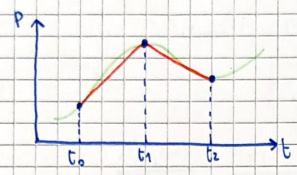
\includegraphics[width=0.5\textwidth]{images/intro_interpolation.png}
        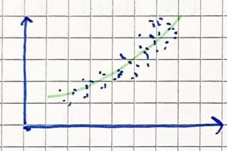
\includegraphics[width=0.45\textwidth]{images/intro_leastsquare.png}
    \end{center}
    Left interpolation, right least square.

    Approximation of functions like integral: approximate it to polynomial. The analytical tool to approximate a function is the Taylor expansion, but it suffers some problems
    \begin{itemize}
        \item Need higher order (more derivatives)
        \item It works well when we consider a neighborhood of the center of the expansion, but moving out of the neighborhood it will start to perform badly
    \end{itemize}

\subsection{Interpolation}
    Instead of Taylor, consider:
    $$
    \begin{bmatrix}
        \text{\textbf{Function}} & & \text{\textbf{Data}}\\
        f & & \Brackets{(x_i,y_i)} \qquad i=0,\cdots,n\\
        y_i=f(x) & & x_i\text{ distinct}
    \end{bmatrix}
    $$
    Identify a function $\tilde{f}$ s.t. $\tilde{f}(x_i)=y_i$ for $i=0,\cdots,n$, \textbf{interpolation conditions}, $n+1$ conditions. The function $\tilde{f}$ can be:
    \begin{itemize}
        \item Polynomial
        \item Trigonometric expansion (Fourier expansion)
        \item Rational
        $$
        \frac{
            a_0+a_1x+\cdots a_px^p
        }{
            b_0+b_1x+\cdots b_qx^q
        }
        $$
    \end{itemize}
    We consider polynomial interpolation

    \subsubsection{Polynomial interpolation}
    \underline{Theorem}: let $\Brackets{x_i,y_i}^n_{i=0}$ ($x_i$ are interpolation nodes, $y_i$ are values to be interpolated) with $x_i$ all distinct. Then $\exists !$ polynomial degree of $\leq n$ (interpolating/interpolation polynomial) s.t. (we guarantee interpolation condition):
    $$
    \underlabel{
        \Pi_n(x_i)=y_i
    }{n+1 conditions}
    \qquad i=0,\cdots,n
    $$
    \underline{Proof for uniqueness}: by contradiction assume that we have 2 interpolating polynomials of order $n$
    $$
    \Pi_n\in\mathbb{P}_n\qquad \Pi_n(x_i)=y_i\qquad i=0,\cdots,n
    $$
    $$
    \Pi_n^*\in\mathbb{P}_n\qquad \Pi_n^*(x_i)=y_i\qquad i=0,\cdots,n
    $$
    Consider the difference
    $$
    D(x)=\Pi_n(x)-\Pi_n^*(x)\in\mathbb{P}_n
    $$
    And
    $$
    D(x_i)=\Pi_n(x_i)-\Pi_n^*(x_i)=y_i-y_i=0\qquad i=0,\cdots,n
    $$
    A polynomial of degree $n$ has at most $n$ intersections with the $x$-axis, but in this case $D(x)$ of degree $n$ has $n+1$ zeros: the only way that we can satisfy the $n+1$ conditions is that $D(x)$ is identically equal to 0. which means
    $$
    D(x)=0\Rightarrow
    \Pi_n(x)-\Pi_n^*(x)=0\Rightarrow
    \Pi_n(x)=\Pi_n^*(x)
    $$
    Which contradicts our initial assumption.

    \underline{Finding the characteristic polynomial}: assume that values to be interpolated are all null except one
    $$
    y_i=0\,\,\forall i\neq k\qquad y_k=1
    $$
    $$
    \begin{Bmatrix}    
        x_0=0 & x_1=0.5 & x_2=1\\
        y_0=0 & y_1=1 & y_2=0
    \end{Bmatrix}
    $$
    Let change notation, instead of $\Pi_2$ we use $\phi_k$
    $$
    \phi_1\in\mathbb{P}_2\qquad
    \underlabel{
        \phi_1(x_0=0)=0
    }{A}\qquad
    \underlabel{
        \phi_1(x_1=1/2)=1
    }{B}\qquad
    \underlabel{
        \phi_1(x_2=1)=0
    }{C}\qquad
    $$
    We want to build a polynomial of degree 2 that is zero in those two points:
    $$
    \begin{cases}
        (x-0)(x-1)\qquad\text{satisfies A and B}\\
        \frac{
            (x-0)(x-1)
        }{
            (0.5-0)(0.5-1)
        }\qquad\text{satisfies C}
    \end{cases}
    $$
    $$
    \phi_1(x)=\cdots=-4x(x-1)
    $$
    With a generic case
    $$
    \phi_k(x_i)=\delta_{ik}=\begin{cases}
        0\qquad i\neq k\\
        1\qquad i=k
    \end{cases}
    $$
    Kronecker delta, to express it as a polynomial with degree $n$, the characteristic polynomial:
    \begin{LARGE}
        $$
        \phi_k(x)=
        \prod_{j=0,j\neq k}^n
        \frac{
            x-x_j
        }{
            x_k-x_j
        }
        $$
    \end{LARGE}
    \underline{Moving to a more general case}: instead of a set of arbitrary values
    $$
    \begin{Bmatrix}
        x_0 & x_1 & x_2\\
        y_0 & y_1 & y_2\\
        \Pi(x_0)=y_0 & \Pi(x_1)=y_1 & \Pi(x_2)=y_2
    \end{Bmatrix}
    $$
    Expressing $\Pi_2$ as linear combination of $\phi_0$, $\phi_1$ and $\phi_2$
    $$
    \begin{Bmatrix}
        \phi_0 & \phi_0(x_0)=1 & \phi_0(x_1)=0 & \phi_0(x_2)=0\\
        \phi_1 & \phi_1(x_0)=0 & \phi_1(x_1)=1 & \phi_1(x_2)=0\\
        \phi_2 & \phi_2(x_0)=0 & \phi_2(x_1)=0 & \phi_2(x_2)=1
    \end{Bmatrix}
    $$
    $$
    \Pi_2(x)=a\phi_0(x)+b\phi_1(x)+c\phi_2(x)
    $$
    Solving we will get:
    $$
    a=y_0\qquad b=y_1\qquad c=y_2
    $$
    The \textbf{Lagrange form}:
    \begin{LARGE}
        $$
        \Pi_n(x)=\sum_{k=0}^ny_k\phi_k(x)
        $$
        $$
        \Pi_n(x)=\sum_{k=0}^ny_k\prod_{j=0,j\neq k}^n
        \frac{
            x-x_j
        }{
            x_k-x_j
        }
        $$
    \end{LARGE}
    In matlab:
    \begin{itemize}
        \item \textbf{c = polyfit(x,y,n)}, to build interpolating polynomial
        \begin{itemize}
            \item x vector collecting interpolation nodes, $x_i$
            \item y is $y_i$
            \item n is the degree of the polynomial, but is redundant as there is a strict relation between number of data and degree of polynomial (for $n$ data, the polynomial will have defree of $n-1$), in least squares it will have a meaning
        \end{itemize}
        It returns the coefficients of our interpolating polynomial
        $$
        p_n(x)=a_nx^n+a_{n-1}x^{n-1}+\cdots+a_1x+a_0
        $$
        With c(1) coefficient of $x^n$, c(2) of $x(n-1)$
        \item \textbf{d = polyval(c,z)}, to evaluate interpolating polynomial at point $z$
        \begin{itemize}
            \item If z single number $\mathbb{R}$, d will be a number
            \item If z is $\mathbb{R}^q$, vector
        \end{itemize}
    \end{itemize}

    \subsubsection{Interpolation error}
    Error at nodes is null, at points that are not nodes? Consider a function continuous in a certain interval $I$:
    $$
    f\in C^0(\overline{I})\qquad I (x_0,x_n)
    $$
    $$
    \Brackets{(x_i,y_i=f(x_i))}^n_{i=0}\qquad x_i\text{ distinct}
    $$
    Assuming
    $$
    f\in C^{n+1}(\overline{I})
    $$
    We define the interpolation error:
    $$
    \forall\,\,x\in\,\,I
    $$
    $$
    E_nf(x)=f(x)-\Pi_nf(x)=\frac{
        f^{(n+1)}\left(\alpha(x)\right)
    }{
        (n+1)!
    }\prod_{k=0}^n (x-x_k)
    $$
    And as expected $E_nf(x_i)=0$. The weak point is that we assume regularity in the function, which depends on the number of nodes: such regularity uncommon. Another drawback is that the $\alpha(x)$ depends on $x$ but we don't know the exact value of $\alpha(x)\in I$. In practice this result useless, so we consider the maximum value.

    If we have more and more information, more samples, the degree of polynomial increases and we have more zeros (the function meets the x axis more times, like sinusoid) but the quality of the approximation improves.\\
    Consider an uniform partition of the interval
    \begin{center}
        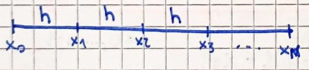
\includegraphics[width=0.7\textwidth]{images/uniform_dist.png}
    \end{center}
    $$
    h=\frac{x_n-x_0}{n}
    $$
    $$
    x_k=x_{k+1}+h\qquad k=1,\cdots,n
    $$
    $$
    x_j=x_0+jh\qquad j=0,\cdots,n
    $$
    In this case we can prove:
    $$
    \left|
        \prod_{k=0}^n(x-x_k)
    \right|\leq
    n!\frac{h^{n+1}}{4}
    $$
    Therefore:
    \begin{LARGE} 
    $$
    \max_{x\in I}\left|E_nf(x)\right|
    \leq
    \underlabel{
        \frac{
            h^{n+1}
        }{
            4(n+1)
        }
    }{A}
    \cdot
    \underlabel{
        \max_{x\in I}\left|
            f^{(n+1)}(x)
        \right|
    }{B}
    $$
    \end{LARGE}
    The two blocks:
    \begin{itemize}
        \item A$\rightarrow$0 for $n\rightarrow\infty$
        \item B for $n\rightarrow\infty$ depends on $f$:
        $$
        \text{B}\rightarrow
        \begin{cases}
            0\\
            \text{constant}\\
            +\infty\begin{cases}
                \text{If A goes to 0 quicker, OK}\\
                \text{If B goes to $\infty$ quicker, not OK}
            \end{cases}
        \end{cases}
        $$
    \end{itemize}
    Consider infact the function
    $$
    f(x)=\frac{1}{1+x^2}\qquad x\in I =\left[-5,5\right]
    $$
    \begin{center}
        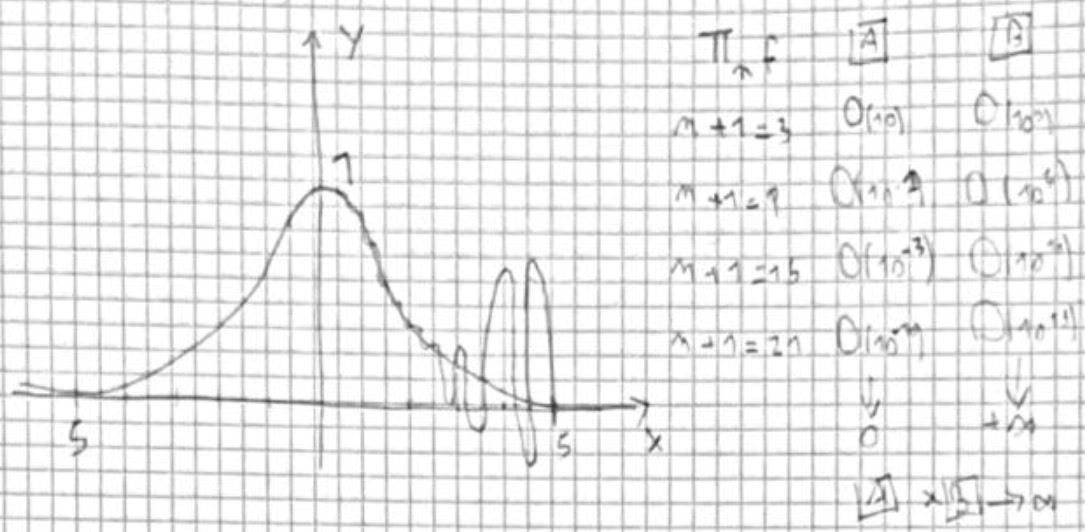
\includegraphics[width=0.9\textwidth]{images/runge.png}
    \end{center}
    We are in presence of spurious oscillations, in the case this error goes to $\infty$, we have the \textbf{Runge phenomenon: more samples, possibility of spurious oscillations}.\\
    To deal with this we can:
    \begin{itemize}
        \item Particular choice of nodes, Chebyshev nodes, as we chose uniform sampling, uniform distribution of nodes, not good idea: with Chebyshev we choose more nodes near the endpoints where the Runge phenomenon occurs, while at the center of the interval less nodes. To divide into $n$ parts:
        \begin{enumerate}
            \item $n$ equal parts first
            $$
            \frac{\Pi_i}{n}\qquad i=0,\cdots,n
            $$
            \item Compute the projection on the x-axis, the minus sign is in order to fix the order
            $$
            -f\left(
                \frac{\Pi_i}{n} 
            \right)
            $$
            \item To use Chebyshev, use the following function that maps the interval $I$ to the generic interval $[a,b]$, maps the nodes of previous step
            $$
            x_i=\frac{a+b}{2}+\frac{b-a}{2}\hat{x}_i
            $$
        \end{enumerate}
        \item When we increase $n$, a lot of x-axis crosses, so we can use low degree polynomials and work interval by interval: \textbf{piecewise linear interpolation}
    \end{itemize}
    
    \subsubsection{Piecewise linear interpolation}
    We do not have to select an uniform distribution of nodes
    $$
    I_j=\left[x_j,x_{j+1}\right]\qquad h_j=x_{j+1}-x_j
    $$
    $$
    H=\max_jh_j
    $$
    The idea is consider each subinterval and replace the function $f$ with conjuction of endpoints (polynomial with low degree, so we avoid oscillations). By increasing the number of nodes, the approximation improves
    \begin{center}
        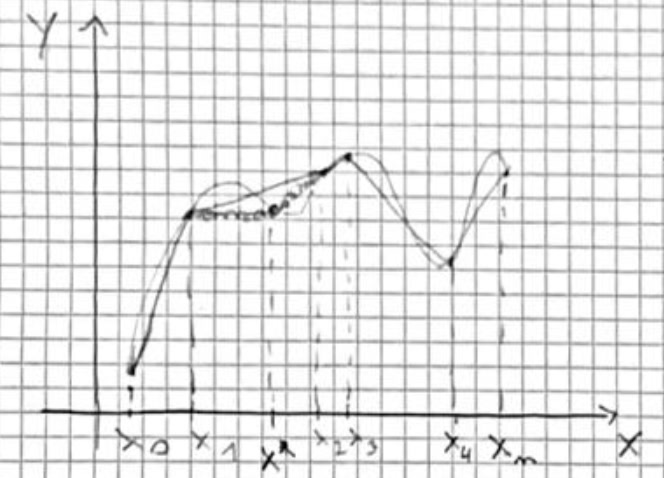
\includegraphics[width=0.7\textwidth]{images/piecewise.png}
    \end{center}
    We indicate linear interpolant as:
    $$
    \Pi_1^Hf\in C^0(\overline{I})
    $$
    $$
    \Pi_1^Hf\Big|_{I_j}\in \mathbb{P}_1(I_j)
    $$
    $$
    \Pi_i^Hf(x_k)=f(x_k)\qquad k=0,\cdots,n
    $$
    Express it as conjuction of endpoints that includes those 3 requirements:
    \begin{LARGE}
        $$
        \Pi_1^Hf(x)=f(x_j)+\frac{
            f(x_{j+1})-f(x_j)
        }{
            x_{j+1}-x_j
        }(x-x_j)\qquad
        x\in I_j
        $$
    \end{LARGE}
    How to prove that the error becomes 0 for $n\rightarrow\infty$? We consider the local error on the subintervals $I_j$, we have (for $n=1$):
    \begin{LARGE}
        $$
        \max_{x\in I_j}\left|E_1^Hf(x)\right|
        \leq
        \frac{
            h_j^2
        }{
            4\cdot(1+1)
        }\cdot
        \max_{x\in I_j}\left|
            f''(x)
        \right|\qquad
        f\in C^2(\overline{I}_j)
        $$
    \end{LARGE}
    Instead of $I_j$ and $h_j$, we want inequality on all $I$:
    \begin{LARGE}
        $$
        \max_{x\in I}\left|E_1^Hf(x)\right|
        \leq
        \frac{
            H^2
        }{
            8
        }\cdot
        \max_{x\in I}\left|
            f''(x)
        \right|\qquad
        f\in C^2(\overline{I})
        $$
    \end{LARGE}
    Now we have the error that is decreasing:
    \begin{itemize}
        \item A = $\frac{H^2}{8}$, for $n\rightarrow\infty$, the maximum length $H$ will become smaller and smaller as we are increasing samples!
        \item B = $\max_{x\in I}\left|f''(x)\right|$ does not change, it's not dependent on $n$
    \end{itemize}
    We can also use piecewise parabola or cubic interpolation, when we join pieces of parabola is the approximation more regular? Is it a $C^1$ or still $C^0$? Not $C^1$, so by increasing local degree of polynomial we do not gain regularity, but we are improving accuracy of approximation. For example $n=2$
    $$
        \max_{x\in I_j}\left|E_2^Hf(x)\right|
        \leq
        \frac{
            h_j^3
        }{
            4\cdot(2+1)
        }\cdot
        \max_{x\in I_j}\left|
            f^{(3)}(x)
        \right|\qquad
        f\in C^3(\overline{I}_j)
    $$
    $$
    \max_{x\in I}\left|E_1^Hf(x)\right|
    \leq
    \frac{
        H^3
    }{
        12
    }\cdot
    \max_{x\in I}\left|
        f^{(3)}(x)
    \right|\qquad
    f\in C^3(\overline{I})
    $$
    This is a problem, we would like something that is globally very smooth.

    In matlab:
    \begin{itemize}
        \item \textbf{d = interp1(x,y,z)}, in some sense merges both polyfit and polyval, output will have same dimension as z
        \item \textbf{d = interp2(x,y,z)}, cubic interpolation
    \end{itemize}
    A remark: the matlab function plot is doing a sampling of the function, which is finer in the gradient of the function. This is known as \textbf{adaptive sampling}

    \subsubsection{Cubic spline interpolation}
    Again, a piecewise interpolation, but we join endpoints with a cubic function
    \begin{enumerate}
        \item $S_3\Big|_{I_j}\in\mathbb{P}$
        \item Spline means function \textbf{smooth globally}, the pieces are joined so that the function is globally, $S_3\in C^2(\overline{I})$
        \item $S_3(x_i)=f(x_i)\qquad i=0,\cdots,n$
    \end{enumerate}
    In matlab \textbf{d = spline(x,y,z)}, build and directly evaluate. For each interval we have a polynomial of degree 3: $S_3$ (so $a_i$ for $i=4$).We have 4 unknowns for each interval, let \#intervals = $n$, so $4n$ unknowns. The procedure:
    \begin{enumerate}[1)]
        \item $S_3((x_i)=f(x_i)\qquad i=0,\cdots,n$
        \item We demand $S_3$ continuous in the nodes, $S_3\in C^0\left(\left[
            x_0,x_n
        \right]\right)$
        $$
        \left[S_3(x_i)\right]^-=
        \left[S_3(x_i)\right]^+
        \qquad i=1,\cdots,n-1
        $$
        \item We demand $S_3'$ continuous in the nodes, $S_3'\in C^0\left(\left[
            x_0,x_n
        \right]\right)$
        $$
        \left[S_3'(x_i)\right]^-=
        \left[S_3'(x_i)\right]^+
        \qquad i=1,\cdots,n-1
        $$
        \item We demand $S_3''$ continuous in the nodes, $S_3''\in C^0\left(\left[
            x_0,x_n
        \right]\right)$
        $$
        \left[S_3''(x_i)\right]^-=
        \left[S_3''(x_i)\right]^+
        \qquad i=1,\cdots,n-1
        $$
    \end{enumerate}
    In total we have $(n+1)+3(n-1)=4n-2$ conditions, but we need two more:
    \begin{itemize}
        \item $S_3''(x_0)=S_3''(x_n)=0$, natural cubic interpolating spline
        \item Not-a-knot-condition: $S_3''$ continuous at $x_1,x_{n-1}$
        $$
        \left[
            S_3'''(x_1)
        \right]^-=
        \left[
            S_3'''(x_1)
        \right]^+
        \qquad
        \left[
            S_3'''(x_{n-1})
        \right]^-=
        \left[
            S_3'''(x_{n-1})
        \right]^+
        $$
    \end{itemize}
    The error:
    $$
    \max_{x\in\left[x_0,x_n\right]}
    \left|
        f^{(r)}(x)-
        S_3^{(r)}(x)
    \right|\leq
    C_r\cdot
    H^{4-r}\cdot
    \max_{x\in\left[x_0,x_n\right]}
    \left|
        f^{(4)}(x)
    \right|
    \qquad r=0,1,2
    $$

\subsection{Least Squared Approximation}
    Data $\Brackets{(x_i,y_i)}^n_{i}$, $x_i$ distinct, we find a polynomial $\tilde{f}\in\mathbb{P}_m$ of degree $m\geq 1,m<<n$ and $\tilde{f}(x_i)\neq y_i$ such that:
    \begin{LARGE}
        $$
        \underlabel{
            \sum_{i=0}^m\left[\tilde{f}(x_i)-y_i\right]^2
        }{A}
        \leq
        \underlabel{
            \sum_{i=0}^n\left[p_m(x_i)-y_i\right]^2
        }{B}
        \qquad\forall\,\,p_m\in\mathbb{P}_m
        $$
    \end{LARGE}
    We want to minimize the right term.
    \subsubsection{Degree n}
    $m=n$ Lagrange interpolant, $\tilde{f}==\Pi_n$

    \subsubsection{Degree 1}
    $m=1$ regression line
    $$
    p_1(x)=b_0+b_1x\qquad b_0,b_1\in\mathbb{R}
    $$
    $$
    \tilde{f}(x)=a_0+a_1x\qquad a_0,a_1\in\mathbb{R}
    $$
    We want to find the specific polynomial $\tilde{f}$ (so the two coefficients). Consider the definition, the blocks:
    \begin{itemize}
        \item A = $\sum_{i=0}^n\left[a_0+a_1x_i-y_i\right]^2=\Phi(a_0,a_1)$
        \item B = $\sum_{i=0}^n\left[b_0+b_1x_i-y_i\right]^2=\Phi(b_0,b_1)$
    \end{itemize}
    So:
    $$
    \Phi(a_0,a_1)\leq\Phi(b_0,b_1)\qquad\forall\,\,b_0,b_1\in\mathbb{R}
    $$
    We compute the partial derivatives to find $a_0$ and $a_1$:
    $$
    \frac{
        \partial\Phi
    }{\partial b_0}\Big|_{(b_0,b_1)=(a_0,a_1)}=0
    \qquad
    \frac{
        \partial\Phi
    }{\partial b_1}\Big|_{(b_0,b_1)=(a_0,a_1)}=0
    $$
    By developing $\Phi(b_0,b_1)$
    $$
    \Phi(b_0,b_1)=
    \sum_{i=0}^n\left[b_0^2+b_1^2x_i^2+y_i^2+2b_0b_1x_i-2b_0y_i-2b_1x_iy_i\right]
    $$
    And the partial derivatives:
    $$
    \frac{
        \partial\Phi
    }{\partial b_0}=\sum_{i=0}^n\left[
        2b_0+2b_1x_i-2y_i
    \right]
    \qquad
    \frac{
        \partial\Phi
    }{\partial b_0}=\sum_{i=0}^n\left[
        2b_1x_i^2+2b_0x_i-2x_iy_i
    \right]
    $$
    Putting $a_0$ and $a_1$
    $$
    \begin{cases}            
        \sum_{i=0}^n\left[
            2a_0+2a_1x_i-2y_i
        \right]=0
        \\
        \sum_{i=0}^n\left[
            2a_1x_i^2+2a_0x_i-2x_iy_i
        \right]=0
    \end{cases}\rightarrow B\overrightarrow{a}=\overrightarrow{f}
    $$
    $$
    \begin{cases}            
        \sum_{i=0}^na_0+\sum_{i=0}^na_1x_i=\sum_{i=0}^ny_i
        \\
        \sum_{i=0}^na_1x_i^2+\sum_{i=0}^na_0x_i=\sum_{i=0}^nx_iy_i
    \end{cases}
    \Rightarrow
    \begin{cases}            
        a_0(n+1)+a_1\sum_{i=0}^nx_i=\sum_{i=0}^ny_i
        \\
        a_1\sum_{i=0}^nx_i^2+a_0\sum_{i=0}^nx_i=\sum_{i=0}^nx_iy_i
    \end{cases}
    $$
    $$
    B=\begin{bmatrix}
        (n+1) & \sum x_i\\
        \sum x_i & \sum x_i^2
    \end{bmatrix}\qquad
    \overrightarrow{f}=\left[
        \sum y_i,\sum x_iy_i
    \right]^T\qquad
    \overrightarrow{a}=\left[
        a_0,a_1
    \right]^T
    $$
    Where $B$ is spd (we can use gradient method)

    \subsubsection{Degree m generic}
    $$
    \tilde{f}(x)=a_0+a_1x+a_2x^2+\cdots+a_mx^m
    $$
    $$
    p_m(x)=b_0+b_1x+b_2x^2+\cdots+b_mx^m
    $$
    $$
    \frac{
        \partial\Phi
    }{b_i}\Big|_{(b_0,b_1,\cdots,b_m)=(a_0,a_1,\cdots,a_m)}=0\qquad i=0,\cdots,m
    $$
    Just like before, we wanto to find $a_0,\cdots,a_m$, after the calculations:
    $$
    B=\begin{bmatrix}
        (n+1) & \sum x_i & \sum x_i^2 & \cdots & \sum x_i^m\\
        \sum x_i & \sum x_i^2 & \sum x_i^3 & \cdots & \sum x_i^{m+1}\\
        \vdots\\
        \sum x_i^m & \sum x_i^{m+1} & \sum x_i^{m+2} & \cdots & \sum x_i^{2m}
    \end{bmatrix}
    $$
    $$
    \overrightarrow{a}=\begin{bmatrix}
        a_0\\
        a_1\\
        \vdots\\
        a_m
    \end{bmatrix}\qquad
    \overrightarrow{f}=\begin{bmatrix}
        \sum y_i\\
        \sum x_iy_i\\
        \vdots\\
        x_i^my_i
    \end{bmatrix}
    $$

\subsection{Numerical Integration}
$$
I(f)=\int_{a}^bf(x)dx\qquad
f\in C^0\left([a,b]\right)
$$
The quadrature rule: approximate a function:
$$
\tilde{I}(f)\simeq I(f)
$$
$$
\tilde{I}(f)=\int_{a}^b\tilde{f}(x)dx\qquad
\tilde{f}(x)\simeq f(x)
$$
The steps:
\begin{itemize}
    \item Subdivide into $M$ intervals, the points are known as quadrature nodes
    \begin{center}
        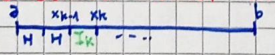
\includegraphics[width=0.5\textwidth]{images/quadrature_nodes.png}
    \end{center}
    $M+1$ points, so $M$ intervals, $x_i$ are quadrature nodes. The amplitude:
    $$
    H=\frac{b-a}{M}
    $$
    Uniform partition of quadrature nodes:
    $$
    x_{i+1}=x_i+H\qquad
    i=0,\cdots,M-1
    $$
    $$
    x_i=x_0+(i)H\qquad i=1,\cdots,M
    $$
    \item Expand the additivity and associativity of integral:
    \begin{LARGE}
        $$
        \int_{a}^bf(x)dx=\sum_{k=1}^M\int_{I_k}f(x)dx\cong
        \sum_{k=1}^M\int_{I_k}\tilde{f}(x)dx=\tilde{I}(f)
        $$
    \end{LARGE}
    With $\tilde{f}(x)\in\mathbb{P}_m$, for different choices of $m$ different quadrature rules
\end{itemize}

\subsubsection{Newton-Cotes}
We have first to define:
\begin{itemize}
    \item \textbf{Order of accuracy}, associated only to the composite rule, "rate of convergence for the quadrature rule to zero- of the error" (it's the power of $H$ in the composite error)
    \item \textbf{Degree of exactness}, associated both to composite and simple, maximum degree of the polynomials which are exactly integrated by your quadrature rule. Suppose:
    $$
    I(f)=\int_a^bf(x)dx\qquad\tilde{I}(f)
    $$
    We start from polynomial of degree 0 $p_0$, but they are infinite: choose a representant
    $$
    I(1)=?=\tilde{I}(1)
    $$
    Then continue till this check does not hold. But in practice the following equality holds:
    $$
    de=\text{[degree of derivative]}-1
    $$
    If we know the explicit expression of the error ($E$) we try different degrees in order to make it zero
\end{itemize}
We have
\begin{itemize}
    \item $m=0$, \textbf{midpoint quadrature rule}, which means for each subinterval $\tilde{f}$ is a constant function
    \begin{center}
        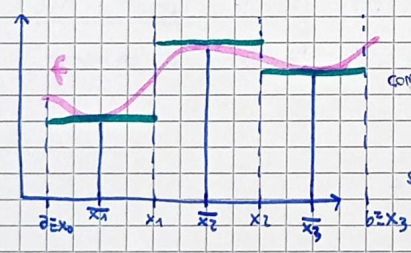
\includegraphics[width=0.5\textwidth]{images/quadrature_m0.png}
    \end{center}
    $$
    \begin{cases}
        \tilde{f}\in\mathbb{P}_0\\
        I_k=[x_{k-1},x_k]\\        
        \overline{x}_k=\frac{x_{k-1}+x_k}{2}
    \end{cases}
    $$
    The composite midpoint quadrature rule:
    \begin{LARGE}
        $$
        \tilde{I}_{MP}^c(f)=H\sum_{k=1}^Mf(\overline{x}_k)
        $$
    \end{LARGE}
    Where $c$ stands for composite, the simple midpoint quadrature rule version:
    $$
    \tilde{I}_{MP}(f)=(b-a)f\left(\frac{a+b}{2}\right)
    $$
    \textbf{Errors}:
    \begin{itemize}
        \item Simple midpoint quadrature rule error
        $$
        I(f)-\tilde{I}_{MP}(f)=\int_a^b\left[f(x)-f(\overline{x})\right]
        $$
        Use the Taylor expansion centered at $\overline{x}$, $f\in C^2([a,b])$, second order:
        $$
        f(x)-f(\overline{x})=f'(\overline{x})(x-\overline{x})+
        \frac{f''(\alpha(x))}{2}(x-\overline{x})^2
        $$
        Making the computations...
        $$
        \tilde{E}_{MP}=I(f)-\tilde{I}_{MP}(f)=
        \frac{(b-a)^3}{24}f''(\beta)
        $$
        $$
        f\in C^2([a,b])\qquad\beta\in[a,b]
        $$
        $\beta$ (from min value theorem of integral) cannot be found, in practice upperbound for worst case
        \item Composite midpoint quadrature rule error
        $$
        I(f)-\tilde{I}_{MP}^c(f)=\sum_{k=1}^M\left[
            \int_{I_k}f(x)dx-
            \tilde{I}_{MP}\left(f\big|_{I_k}\right)
        \right]=
        \sum_{k=1}^M\frac{H^3}{24}f''(\beta_k)
        $$
        Again from min value theorem of summation (dual of integral one):
        $$
        =\frac{H^3}{24}f''(\gamma)\sum_{k=1}^M1=
        =\frac{H^3}{24}f''(\gamma)M=
        $$
        With $H=\frac{b-a}{M}\rightarrow M=\frac{b-a}{M}$, so:
        $$
        \tilde{E}_{MP}^c=I(f)-\tilde{I}_{MP}^c(f)=
        \frac{(b-a)}{24}H^2f''(\gamma)
        $$
        $$
        f\in C^2([a,b])\qquad\gamma\in[a,b]
        $$
    \end{itemize}
    \textbf{Order of accuracy}: $oa_{MP}=2$\\
    \textbf{Degree of exactness}: $de_{MP}=1$
    \begin{itemize}
        \item $p_0$ degree 0
        $$I(1)=?=\tilde{I}(1)$$
        $$
        (b-a)=?=(b-a)f\left(\frac{a+b}{2}\right)=(b-a)
        $$
        OK
        \item $p_1$ degree 1
        $$I(x)=?=\tilde{I}(x)$$
        $$
        \frac{x^2}{2}\Big|_a^b=?=(b-a)\frac{a+b}{2}
        $$
        OK, make the computations
        \item $p_1$ degree 2
        $$I(x^2)=?=\tilde{I}(x^2)$$
        $$
        \frac{x^3}{3}\Big|_a^b=?=(b-a)\left[\frac{a+b}{2}^2\right]
        $$
        KO, we stop here, so $de_{MP}=1$
    \end{itemize}

    \item $m=1$, \textbf{trapezoidal quadrature rule}, for each subinterval a linear function
    \begin{center}
        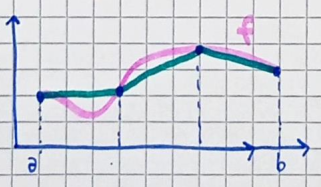
\includegraphics[width=0.5\textwidth]{images/quadrature_m1.png}
    \end{center}
    The composite trapezoidal quadrature rule (just basis times height):
    \begin{LARGE}
        $$
        \tilde{I}_{T}^c(f)=
        \frac{H}{2}
        \sum_{k=1}^M
        \left[
            f(x_{k-1})+f(x_k)
        \right]=
        \frac{H}{2}
        \left[
            f(a)+f(b)
        \right]+
        H\sum_{k=1}^{M-1}f(x_k)
        $$
    \end{LARGE}
    The first expression associated to intervals, the second to nodes. The simple trapezoidal quadrature rule version:
    $$
    \tilde{I}_T(f)=\frac{(b-a)}{2}\left[f(a)+f(b)\right]
    $$
    \textbf{Errors}:
    \begin{itemize}
        \item Simple trapezoidal quadrature rule
        $$
        I(f)-\tilde{I}_T(f)=\int_a^b\left[d(x)-\Pi_1(f)(x)\right]dx
        $$
        The term inside the integral is:
        $$
        E_1=\frac{f''(\eta(x))}{2}(x-a)(a-b)
        $$
        From
        $$
        E_nf(x)=\frac{f^{(n+1)}(\alpha(x))}{(n-1)!}\prod_{k=0}^n(x-x_k)
        $$
        Making the computations...
        $$
        \tilde{E}_T=I(f)-\tilde{I}_T(f)=
        -\frac{(b-a)^3}{12}f''(\delta)
        $$
        $$
        f\in C^2([a,b])\qquad\delta\in[a,b]
        $$
        \item Composite trapezoidal quadrature rule
        $$
        \tilde{E}_T=I(f)-\tilde{I}_T^c(f)=
        -\frac{(b-a)}{12}H^2f''(\rho)
        $$
        $$
        f\in C^2([a,b])\qquad\rho\in[a,b]
        $$
    \end{itemize}
    \textbf{Order of accuracy}: $oa_{T}=2$\\
    \textbf{Degree of exactness}: $de_{T}=1$\\
    Though $oa$ and $de$ same as midpoint, we see that the error is twice that of the midpoint: midpoint is easier and has lower error
    \item $m=2$, \textbf{Simpson quadrature rule}
    \begin{center}
        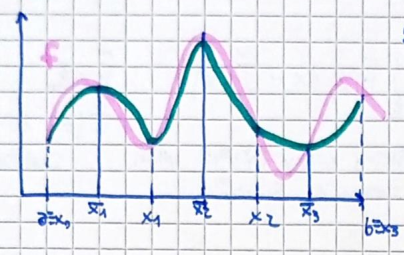
\includegraphics[width=0.5\textwidth]{images/quadrature_m2.png}
    \end{center}
    \begin{LARGE}
        $$
        \tilde{I}_{S}^c(f)=
        \frac{H}{6}
        \sum_{k=1}^M
        \left[
            f(x_{k-1})+4f(\overline{x}_k)+f(x_k)
        \right]=
        $$
        $$
        =
        \frac{H}{6}
        \left[f(a)+f(b)\right]+
        \frac{H}{3}
        \sum_{k=1}^{M-1}f(x_k)+
        \frac{2}{3}H
        \sum_{k=1}^{M}f(\overline{x}_k)
        $$
    \end{LARGE}
    The simple Simpson quadrature rule version:
    $$
    \tilde{I}_S(f)=\frac{(b-a)}{6}\left[
        f(a)+
        4f\left(\frac{a+b}{2}\right)+f(b)
    \right]
    $$

\end{itemize}
\pagebreak
\begin{figure}[!ht]
    \begin{minipage}{\linewidth}
        \centering
        \makebox[\textwidth][c]{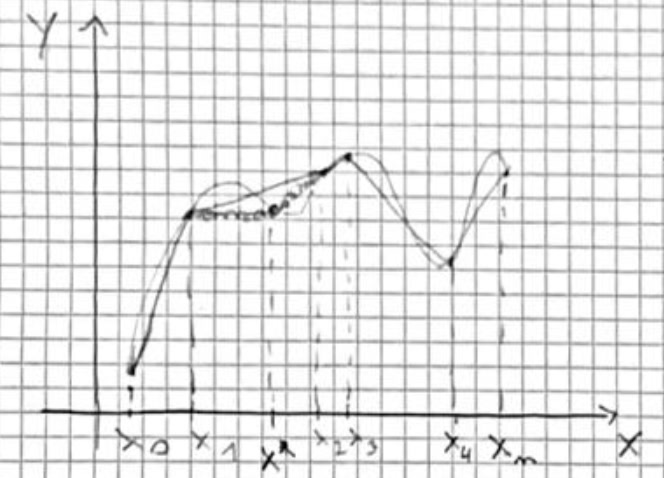
\includegraphics[width=0.8\textwidth]{images/piecewise.png}}%
        \caption{Modified Newton graph}
        %\label{BarsNielsenCrop}
    \end{minipage}
\end{figure}

\begin{center}
    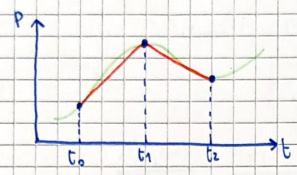
\includegraphics[width=0.5\textwidth]{images/intro_interpolation.png}
    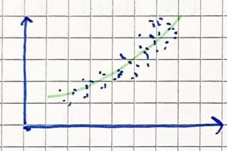
\includegraphics[width=0.45\textwidth]{images/intro_leastsquare.png}
\end{center}

\begin{center}
    \begin{lstlisting}[escapeinside=`']
        while(true)
            `$x^{(k)}=(a^{(k)}+b^{(k)})/2$'
            if(`$f(x^{(k-1)})=0$') break;
            if `$f(a^{(k-1)})f(x^{(k-1)})<0$'
                `$a^{(k)}=a^{(k-1)},b^{(k)}=x^{(k-1)}$';
            else
                `$a^{(k)}=x^{(k-1)},b^{(k)}=b^{(k-1)}$';
            end
        \end{lstlisting}
\end{center}
\begin{center}
    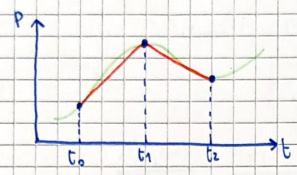
\includegraphics[width=0.5\textwidth]{images/intro_interpolation.png}
\end{center}

    % !TeX root = ../main.tex

\section{Code}

\subsection{Vanilla box}
\fbox{\begin{minipage}{\linewidth}
    \begin{addmargin}[0em]{0em}
        \textbf{Input}: dataset $x_n\in\mathbb{R}^D$\\
        $t_n\in\{-1,+1\}$, for $n=1:N$\\
        Initialize $w_0$\\
        $k\leftarrow 0$\\
        \textbf{repeat}
        \begin{addmargin}[1em]{0em}
            $k\leftarrow k+1$\\
            $n\leftarrow k$ mode $N$\\
            \textbf{if} $\hat{t}_n\neq t_n$ \textbf{then}
            \begin{addmargin}[1em]{0em}
                $w_{k+1}\leftarrow w_k+\phi(x_n)t_n$
            \end{addmargin}
            \textbf{end if}
        \end{addmargin}
        \textbf{until} convergence
    \end{addmargin}    
\end{minipage}}
    %% !TeX root = ../main.tex

\section{Pictures}

\subsection{Simplest centered}
\begin{figure}[!ht]
    \begin{minipage}{\linewidth}
        \centering
        \makebox[\textwidth][c]{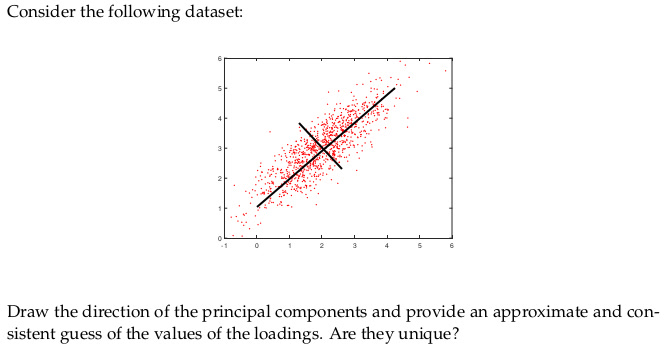
\includegraphics[width=1\textwidth]{images/Bias-Variance Tradeoff_01.png}}%
        %\caption{Nielsen's heuristics evaluation summary}
        %\label{BarsNielsenCrop}
    \end{minipage}
\end{figure}

\subsection{Adjacent centered}
\begin{center}
    
\includegraphics[width=0.3\textwidth]{images/Bias-Variance Tradeoff_03.png}
    \hspace{1em}
    
\includegraphics[width=0.3\textwidth]{images/Bias-Variance Tradeoff_04.png}
\end{center}

\subsection{Captioned figure}
I'm referring to figure \ref{refer_sample}
\begin{figure}[!ht]
    \begin{minipage}[c]{\linewidth}
        \centering
        \makebox[\textwidth][c]{
\includegraphics[width=0.6\textwidth]{images/Bias-Variance Tradeoff_02.png}}%
        \captionsetup{justification=centering}
        \caption{This is a caption}
        \label{refer_sample}
    \end{minipage}
\end{figure}

\subsection{One caption per multiple images}
I'm referring to figure \ref{refer_sample_2}
\begin{figure}[!ht]
    \centering
    \subfloat[][\centering Case 1]{{
\includegraphics[width=7cm]{images/Bias-Variance Tradeoff_03.png} }}%
    \qquad
    \subfloat[][\centering Case 2]{{
\includegraphics[width=7cm]{images/Bias-Variance Tradeoff_04.png} }}%
    \captionsetup{justification=centering}
    \caption{VC dimension < 5}%
    \label{refer_sample_2}%
\end{figure}
\end{document}